%%%%%%%%%%%%%%%%%%%%%%%%%%%%%%%%%%%%%%%%%%%%%%%%%%%%%%%%%%%%%%%%%%%%%%%%%%%%%%%%%%%%%%%%%%%%%%%%%%%
%\documentclass[11pt,mathserif]{beamer}
\documentclass[serif,mathserif,professionalfont]{beamer}
\usetheme[block=fill,progressbar=frametitle]{metropolis}
\usepackage[T1]{fontenc}
\usepackage[utf8]{inputenc}
\usepackage[spanish]{babel}
\usepackage{amsmath}
\usepackage{amsfonts}
\usepackage{amssymb}
\usepackage{graphicx}

% numeros con punto decimal, no coma
\decimalpoint

% para la bibliografia
\usepackage[style=verbose,backend=bibtex]{biblatex}
\bibstyle{abbrv}

% codigo de R
\usepackage{listings}
\usepackage{color}

% para las tablitas
\usepackage{booktabs}

% para tablas de colores
\usepackage{xcolor,colortbl}
\usepackage{multirow}

%\usefonttheme[onlymath]{mathserif}
%\usepackage{mathpazo} 
%\usepackage[scaled ]{helvet}  
%\usepackage{concmath}

\usepackage{pxfonts}
\usepackage{eulervm}


% intento de incluir animaciones
\usepackage{movie15}

%%%%%%%%%%%%%%%%%%%%%%%%%%%%%%%%%%%%%%%%%%%%%%%%%%%%%%%%%%%%%%%%%%%%%%%%%%%%%%%%%%%%%%%%%%%%%%%%%%%

% parametros de sweave
%\SweaveOpts{concordance=TRUE}

%%%%%%%%%%%%%%%%%%%%%%%%%%%%%%%%%%%%%%%%%%%%%%%%%%%%%%%%%%%%%%%%%%%%%%%%%%%%%%%%%%%%%%%%%%%%%%%%%%%

% retoques graficos para el codigo en R
\newsavebox{\caja}

%%%%%%%%%%%%%%%%%%%%%%%%%%%%%%%%%%%%%%%%%%%%%%%%%%%%%%%%%%%%%%%%%%%%%%%%%%%%%%%%%%%%%%%%%%%%%%%%%%%

% comandos para tablas
\newcommand{\bordes}[1]{\renewcommand{\arraystretch}{#1}}
\definecolor{gray}{rgb}{0.5,0.5,0.5}
\definecolor{gris}{gray}{0.925}
\definecolor{gris2}{gray}{0.8}

%%%%%%%%%%%%%%%%%%%%%%%%%%%%%%%%%%%%%%%%%%%%%%%%%%%%%%%%%%%%%%%%%%%%%%%%%%%%%%%%%%%%%%%%%%%%%%%%%%%

% bibliografia
\addbibresource{referencias_estacionariedad.bib}
\addbibresource{referencias_fisiologia.bib}
\addbibresource{referencias_otros.bib}
\addbibresource{referencias_mixto.bib}

\renewcommand{\footnotesize}{\tiny}

%%%%%%%%%%%%%%%%%%%%%%%%%%%%%%%%%%%%%%%%%%%%%%%%%%%%%%%%%%%%%%%%%%%%%%%%%%%%%%%%%%%%%%%%%%%%%%%%%%%

\newtheorem{definicion}{Definición}
\newtheorem{teorema}{Teorema}
\newtheorem{proposicion}{Proposición}
\newtheorem{demostracion}{Demostración}

\newcommand{\R}{\mathbb{R}}
\newcommand{\C}{\mathbb{C}}
\newcommand{\N}{\mathbb{N}}
\newcommand{\Z}{\mathbb{Z}}
\newcommand{\intR}{\int_{-\infty}^{\infty}}
\newcommand{\intZ}{\int_{-\infty}^{0}}
\newcommand{\intPI}{\int_{-\pi}^{\pi}}
\newcommand{\simint}[1]{\int_{- #1 }^{ #1 }}
\newcommand{\prima}{^{\prime}}

\newcommand{\ddd}{$\delta$}
\newcommand{\dirac}{$\delta$  de Dirac}

\newcommand{\aste}[1]{\widehat{ #1 }^{\star}}
\newcommand{\est}[1]{\widehat{ #1 }}

\newcommand{\COS}[1]{\mathrm{cos}\left( #1 \right)}
\newcommand{\SEN}[1]{\mathrm{sen}\left( #1 \right)}

\newcommand{\E}[1]{\mathrm{E}\left[ #1 \right]}
\newcommand{\Var}[1]{\mathrm{Var}\left( #1 \right)}
\newcommand{\Cov}[1]{\mathrm{Cov}\left( #1 \right)}
\newcommand{\abso}[1]{\left| #1 \right|}

\newcommand{\xt}{$\{X(t)\}_{t\in \boldsymbol{T}}$ }
\newcommand{\xtd}{$\{x_t\}_{t=0,\dots,N}$ }
\newcommand{\orden}{\mathcal{O}}

\newcommand{\talque}{\mathrel{}\middle|\mathrel{}}

\newcommand{\lp}{\ell^{p}}
\newcommand{\llp}{L^{p}[I]}
\newcommand{\ldos}{\ell^{2}}
\newcommand{\lldos}{L^{2}[I]}

\newcommand{\sip}{\ding{51}}
\newcommand{\nop}{\ding{55}}

\newcommand{\pz}{\phantom{.0}}
\newcommand{\ppu}{\phantom{1}}
\newcommand{\phm}{\phantom{-}}

\newcommand{\hz}{\si{\hertz}}
\newcommand{\mv}{\si{\micro\volt}}

%%%%%%%%%%%%%%%%%%%%%%%%%%%%%%%%%%%%%%%%%%%%%%%%%%%%%%%%%%%%%%%%%%%%%%%%%%%%%%%%%%%%%%%%%%%%%%%%%%%

% titulo y fecha
\author{Julio Cesar Enciso Alva}
\title{Estacionariedad débil en registros polisomnográficos}
\subtitle{Como marcador de posible deterioro cognitivo en adultos mayores}
%\setbeamercovered{transparent} 
\setbeamertemplate{navigation symbols}{} 
%\logo{} 
\institute{Instituto de Ciencias Básicas e Ingeniería\\ 
Universidad Autónoma del Estado de Hidalgo} 
%\date{\emph{Neuroscience Short Course}\\
%Noviembre de 2017} 
\date{Enero de 2018}
%\subject{} 

%%%%%%%%%%%%%%%%%%%%%%%%%%%%%%%%%%%%%%%%%%%%%%%%%%%%%%%%%%%%%%%%%%%%%%%%%%%%%%%%%%%%%%%%%%%%%%%%%%%

\begin{document}

%\metroset{background=dark}

\begin{frame}
\titlepage
\end{frame}

%\begin{frame}
%\tableofcontents
%\end{frame}

%\metroset{background=light}

%%%%%%%%%%%%%%%%%%%%%%%%%%%%%%%%%%%%%%%%%%%%%%%%%

%\section{Introducción}

\section{Introducci\'on}

%%%%%%%%%%%%%%%%%%%%%%%%%%%%%%%%%%%%%%%%%%%%%%%%%%%%%%%%%%%%%%%%%%%%%%%%%%%%%%%%%%%%%%%%%%%%%%%%%%%

\subsection{Antecedentes}

\begin{frame}\frametitle{Antecedentes}
\begin{itemize}
\item Encuesta Intercensal 2015 (INEGI): 12,500,000 adultos mayores, 10.4 \%  de la poblaci\'on 
\footcite{Intercensal15}

\item Posible relaci\'on trastornos del sue\~no y DC en la vejez \footcite{Miyata13}

\item Epidemiolog\'ia del DC en Hidalgo: eficiencia del sue\~no \footcite{VazquezTagle16}

%\item DFA en registros de PSG \footcite{Valeria}: exponente de Hurst diferente en sujetos con y 
%sin DC 

\item Se buscan marcadores cl\'inicos para el diagn\'ostico de DC
\end{itemize}
\end{frame}

%%%%%%%%%%%%%%%%%%%%%%%%%%%%%%%%%%%%%%%%%%%%%%%%%%%%%%%%%%%%%%%%%%%%%%%%%%%%%%%%%%%%%%%%%%%%%%%%%%%
%%%%%%%%%%%%%%%%%%%%%%%%%%%%%%%%%%%%%%%%%%%%%%%%%%%%%%%%%%%%%%%%%%%%%%%%%%%%%%%%%%%%%%%%%%%%%%%%%%%

\subsection{Objetivos}

\begin{frame}\frametitle{Pregunta de investigaci\'on}
\textbf{
¿Las caracterizaci\'on de registros de PSG como 
series de tiempo d\'ebilmente estacionarias, puede ser usada como marcador diagn\'ostico 
del deterioro cognitivo en adultos mayores?
}
\end{frame}

%%%%%%%%%%%%%%%%%%%%%%%%%%%%%%%%%%%%%%%%%%%%%%%%%%%%%%%%%%%%%%%%%%%%%%%%%%%%%%%%%%%%%%%%%%%%%%%%%%%
%%%%%%%%%%%%%%%%%%%%%%%%%%%%%%%%%%%%%%%%%%%%%%%%%%%%%%%%%%%%%%%%%%%%%%%%%%%%%%%%%%%%%%%%%%%%%%%%%%%
%%%%%%%%%%%%%%%%%%%%%%%%%%%%%%%%%%%%%%%%%%%%%%%%%%%%%%%%%%%%%%%%%%%%%%%%%%%%%%%%%%%%%%%%%%%%%%%%%%%

\section{Conceptos}

%%%%%%%%%%%%%%%%%%%%%%%%%%%%%%%%%%%%%%%%%%%%%%%%%%%%%%%%%%%%%%%%%%%%%%%%%%%%%%%%%%%%%%%%%%%%%%%%%%%

\subsection{Matem\'aticas}

\begin{frame}\frametitle{Conceptos}
\begin{definicion}[Estacionariedad d\'ebil]
Un proceso estoc\'astico es d\'ebilmente estacionario si y s\'olo si para cualesquiera tiempos 
admisibles $t$, $s$ se tiene que
\begin{itemize}
\item $\E{X(t)} = \mu_X$
\item $\Var{X(t)} = \sigma^{2}_X$
\item $\Cov{X(t),X(s)} = \rho_X (s-t)$
\end{itemize}
Con $\mu_X$, $\sigma^{2}_X$ constantes, $\rho_X(\tau)$ \'unicamente depende de $\tau$
\end{definicion}
\end{frame}

%%%%%%%%%%%%%%%%%%%%%%%%%%%%%%%%%%%%%%%%%%%%%%%%%
%%%%%%%%%%%%%%%%%%%%%%%%%%%%%%%%%%%%%%%%%%%%%%%%%

\begin{frame}\frametitle{Conceptos}
%\begin{definicion}[Continuidad estoc\'astica en media cuadr\'atica]
%Un proceso a tiempo continuo $\{ X(t) \}$ es estoc\'asticamente continuo en $t_0$ si y s\'olo si
%\begin{equation*}
%\lim_{t \rightarrow t_0} \E{\left( X\left(t\right) - X\left(t_0\right) \right)^{2}} = 0
%\end{equation*}
%\end{definicion}

\begin{definicion}[Funci\'on de densidad espectral, FDE]
Sea $\{X(t)\}$ un proceso estoc\'astico a tiempo continuo, d\'ebilmente estacionario
\begin{equation*}
h(\omega) = \lim_{T\rightarrow \infty} \E{ \frac{ \left| G_T(\omega) \right|^{2}}{2 T} }
\end{equation*}
Donde $\displaystyle G_T (\omega) = \frac{1}{\sqrt{2 \pi}} \int_{-T}^{T} X(t) e^{-i \omega t} dt$
\end{definicion}
\end{frame}

%%%%%%%%%%%%%%%%%%%%%%%%%%%%%%%%%%%%%%%%%%%%%%%%%
%%%%%%%%%%%%%%%%%%%%%%%%%%%%%%%%%%%%%%%%%%%%%%%%%

\begin{frame}\frametitle{FDE vs Autocorrelación}
\begin{teorema}[Wiener-Khinchin]
Una condici\'on suficiente y necesaria para que $\rho$ sea funci\'on de autocorrelaci\'on para 
alg\'un proceso a tiempo continuo d\'ebilmente estacionario y estoc\'asticamente continuo, 
$\{X(t)\}$,  es que exista una funci\'on $F$ tal que
\begin{itemize}
\item Es mon\'otonamente creciente
\item $F(-\infty) = 0$
\item $F(+\infty) = 1$
\item Para todo $\tau \in \R$ se cumple que
\begin{equation*}
\rho(\tau) = \intR e^{i \omega \tau} dF(\omega)
\end{equation*}
\end{itemize}
\end{teorema}
\end{frame}

%%%%%%%%%%%%%%%%%%%%%%%%%%%%%%%%%%%%%%%%%%%%%%%%%
%%%%%%%%%%%%%%%%%%%%%%%%%%%%%%%%%%%%%%%%%%%%%%%%%

\begin{frame}\frametitle{Representaci\'on de Wold-Cram\'er}
\begin{teorema}
Sea $\{X(t)\}$ un proceso a tiempo continuo, d\'ebilmente estacionario, estoc\'asticamente 
continuo, de media 0 y varianza finita. Entonces, existe un proceso ortogonal $\{Z(\omega)\}$ tal 
que
\begin{equation*}
X(t) = \intR e^{i t \omega} dZ(\omega)
\end{equation*}
El proceso $\{Z(t)\}$ cumple para todo $\omega$
\begin{itemize}
\item $\E{dZ(\omega)} = 0$
\item $\E{\abso{dZ(\omega)}^{2}} = dH(\omega)$
\item $\Cov{dZ(\omega),dZ(\lambda)} = 0 \Leftrightarrow \omega \neq \lambda$
\end{itemize}
Con $H$ la SDF integrada de $\{X(t)\}$
\end{teorema}
\end{frame}

\begin{frame}\frametitle{Espectro evolutivo}
Se consideran procesos no-estacionarios, estoc\'asticamente continuos, de media cero y varianza 
finita, y que admitan una representaci\'on de la forma
\begin{equation*}
X(t) = \intPI A(t,\omega) e^{i t \omega} dZ(\omega)
\end{equation*}
tal que 
\begin{itemize}
\item $\Cov{dZ(\omega),dZ(\lambda)} = 0 \Leftrightarrow \omega \neq \lambda$
\item $\E{\abso{dZ(\omega)}^{2}} = \mu(\omega)$
\end{itemize}

El \textbf{espectro evolutivo} fue definido por Priestley \footcite{Priestley65} como
\begin{equation*}
f(t,\omega) = \abso{A(t,\omega)}^{2}
\end{equation*}
\end{frame}

%%%%%%%%%%%%%%%%%%%%%%%%%%%%%%%%%%%%%%%%%%%%%%%%%
%%%%%%%%%%%%%%%%%%%%%%%%%%%%%%%%%%%%%%%%%%%%%%%%%

\begin{frame}%\frametitle{Estimador de doble ventana}
\begin{definicion}[Estimador de doble ventana]
Se define a $\est{f}$, estimador para la $f$, como
\begin{equation*}
\widehat{f}(t,\omega) = \int_{t-T}^{t} w_{T'}(u) \lvert U(t-u,\omega) \lvert^{2} du
\end{equation*}

\begin{itemize}
\item $U(t,\omega) = \int_{t-T}^{t} g(u) X({t-u}) e^{i \omega (t-u)} du$

\item $2\pi \int_{-\infty}^{\infty} \lvert g(u) \lvert^{2} du = 
\int_{-\infty}^{\infty} \lvert \Gamma(\omega) \lvert^{2} d\omega = 1$
\item $w_{\tau}(t) \geq 0$ para cualesquiera $t$, $\tau$
\item $w_{\tau}(t) \rightarrow 0$ cuando $\lvert t \lvert \rightarrow \infty$, para todo $\tau$
\item $\int_{-\infty}^{\infty} w_{\tau}(t) dt = 1$ para todo $\tau$
\item $ \int_{-\infty}^{\infty} \left( w_{\tau}(t) \right)^{2} dt < \infty$ para todo $\tau$
\item $\exists C$ tal que  
$ \lim_{\tau\rightarrow\infty} \tau \int_{-\infty}^{t} \abso{ W_{\tau}(\lambda) }^{2} d\lambda = C$
\end{itemize}
\end{definicion}
\end{frame}

%%%%%%%%%%%%%%%%%%%%%%%%%%%%%%%%%%%%%%%%%%%%%%%%%
%%%%%%%%%%%%%%%%%%%%%%%%%%%%%%%%%%%%%%%%%%%%%%%%%

%\begin{frame}%\frametitle{}
%\begin{proposicion}
%El estimador de doble ventana $\widehat{f}$ tiene las siguientes propiedades
%\begin{itemize}
%\item $\displaystyle \E{\est{f}(t,\omega)} \approx f(t,\omega)$
%\item $\displaystyle \Var{\est{f}(t,\omega)} \approx 
%\frac{C}{\tau} f^{2}(t,\omega) \intR \abso{\Gamma (\theta)}^{4} d\theta$
%\item $\displaystyle \Cov{\est{f}(t_1,\omega_1) , \est{f}(t_2,\omega_2)} \approx \intR \intR
%w_\tau (u) w_\tau(v) \Cov{ \abso{U(t_1-u,\omega_1)}^{2} , \abso{U(t_2-u,\omega_2)}^{2} } du dv$
%\end{itemize}
%\end{proposicion}
%
%\begin{proposicion}
%El estimador $ Y(t,\omega) = \log{\left( \est{f}(t,\omega)\right)}$ satisface que
%\begin{itemize}
%\item $\displaystyle 
%\E{ Y(t,\omega) } \approx \log \left( f(t,\omega) \right)$
%\item $\displaystyle 
%\Var{ Y(T,\omega) } 
%\approx \frac{C}{\tau} \intR \abso{\Gamma (\theta)}^{4} d\theta $
%\end{itemize}
%\end{proposicion}
%\end{frame}

\begin{frame}
\begin{proposicion}
El estimador $ Y(t,\omega) = \log{\left( \est{f}(t,\omega)\right)}$ satisface que
\begin{itemize}
\item $\displaystyle 
\E{ Y(t,\omega) } \approx \log \left( f(t,\omega) \right)$
item $\displaystyle 
\Var{ Y(T,\omega) } 
\approx \frac{C}{\tau} \intR \abso{\Gamma (\theta)}^{4} d\theta $
\end{itemize}
\end{proposicion}

M\'as a\'un, puede escribirse
\begin{equation*}
Y(t,\omega) = \log \left( f(t,\omega) \right) + \varepsilon(t,\omega)
\end{equation*}
donde las variables $\varepsilon(t,\omega)$ satisfacen que
\begin{itemize}
\item $\displaystyle \E{\varepsilon(t,\omega)} = 0$
\item $\displaystyle \Var{\varepsilon(t,\omega)}
\approx \frac{C}{\tau} \intR \abso{\Gamma (\theta)}^{4} d\theta$
\end{itemize}
\end{frame}

%%%%%%%%%%%%%%%%%%%%%%%%%%%%%%%%%%%%%%%%%%%%%%%%%
%%%%%%%%%%%%%%%%%%%%%%%%%%%%%%%%%%%%%%%%%%%%%%%%%

%\begin{frame}%\frametitle{}
%M\'as a\'un, puede escribirse
%\begin{equation*}
%Y(t,\omega) = \log \left( f(t,\omega) \right) + \varepsilon(t,\omega)
%\end{equation*}
%donde las variables $\varepsilon(t,\omega)$ satisfacen que
%\begin{itemize}
%\item $\displaystyle \E{\varepsilon(t,\omega)} = 0$
%\item $\displaystyle \Var{\varepsilon(t,\omega)}
%\approx \frac{C}{\tau} \intR \abso{\Gamma (\theta)}^{4} d\theta$
%\end{itemize}
%
%En particular, se puede usar num\'ericamente el que
%\begin{equation*}
%\sum_{i = 1 }^{N} \left( Y(t,\omega_i) - \overline{Y}(\bullet,\omega_i) \right)^{2} 
%\sim \sigma^{2} \chi^{2}(N)
%\end{equation*}
%con $\sigma^{2} = \Var{\varepsilon(t,\omega)}$, y
%$\overline{Y}(\bullet,\omega) = \frac{1}{M} \sum_{j=1}^{M} Y(t_j,\omega)$.
%\end{frame}

%%%%%%%%%%%%%%%%%%%%%%%%%%%%%%%%%%%%%%%%%%%%%%%%%
%%%%%%%%%%%%%%%%%%%%%%%%%%%%%%%%%%%%%%%%%%%%%%%%%

%\begin{lrbox}{\mybox}%
%\begin{lstlisting}[caption={}]
%Priestley-Subba Rao stationarity Test for datos
%-----------------------------------------------
%Samples used              : 3072 
%Samples available         : 3069 
%Sampling interval         : 1 
%SDF estimator             : Multitaper 
%  Number of (sine) tapers : 5 
%  Centered                : TRUE 
%  Recentered              : FALSE 
%Number of blocks          : 11 
%Block size                : 279 
%Number of blocks          : 11 
%p-value for T             : 0.4130131 
%p-value for I+R           : 0.1787949 
%p-value for T+I+R         : 0.1801353 
%\end{lstlisting}
%\end{lrbox}%
%
%\begin{frame}[fragile]
%\begin{figure}
%\scalebox{0.8}{\usebox{\mybox}}
%\caption{La prueba de Priestley-Subba Rao se encuentra implementada en R como la funci\'on 
%\texttt{stationarity()}, del paquete \texttt{fractal}}
%\end{figure}
%\end{frame}

%%%%%%%%%%%%%%%%%%%%%%%%%%%%%%%%%%%%%%%%%%%%%%%%%%%%%%%%%%%%%%%%%%%%%%%%%%%%%%%%%%%%%%%%%%%%%%%%%%%
%%%%%%%%%%%%%%%%%%%%%%%%%%%%%%%%%%%%%%%%%%%%%%%%%%%%%%%%%%%%%%%%%%%%%%%%%%%%%%%%%%%%%%%%%%%%%%%%%%%

\section{Metodolog\'ia}

%%%%%%%%%%%%%%%%%%%%%%%%%%%%%%%%%%%%%%%%%%%%%%%%%%%%%%%%%%%%%%%%%%%%%%%%%%%%%%%%%%%%%%%%%%%%%%%%%%%

\subsection{Participantes}

%%%%%%%%%%%%%%%%%%%%%%%%%%%%%%%%%%%%%%%%%%%%%%%%%
%%%%%%%%%%%%%%%%%%%%%%%%%%%%%%%%%%%%%%%%%%%%%%%%%

\begin{frame}\frametitle{Sujetos}
Criterios de inclusi\'on:
\begin{itemize}
\item Firma del consentimiento informado
\item Edad entre 60 y 85 a\~nos
\item Diestros (mano derecha dominante)
\item Sin ansiedad, depresi\'on o s\'indromes focales
\item No usar medicamentos o sustancias para dormir
\item Voluntario para el registro de PSG
\end{itemize}

\textbf{10 participantes: 5 CTL, 5 PDC}
\end{frame}

%%%%%%%%%%%%%%%%%%%%%%%%%%%%%%%%%%%%%%%%%%%%%%%%%
%%%%%%%%%%%%%%%%%%%%%%%%%%%%%%%%%%%%%%%%%%%%%%%%%

\begin{frame}\frametitle{Participantes}
\begin{table}
\centering
\bordes{1.1}
\begin{tiny}
\begin{tabular}{llcrrrrrrr}
\toprule
 \phantom{.}&
 & {Sexo} & {Edad} & {Escol.} & {Neuropsi} & {MMSE} & {SATS} & {KATZ} & {GDS} \\
\midrule
\multicolumn{6}{l}{\textbf{Grupo CTL}}\\
&VCR    & F    & 59\pz & 12\pz & 107\pz & 29\pz & 21\pz & 0\pz & 3\pz \\
&MJH    & F    & 72\pz & 9\pz  & 113\pz & 30\pz & 18\pz & 0\pz & 0\pz \\
&JAE    & F    & 78\pz & 5\pz  & 102\pz & 28\pz & 19\pz & 0\pz & 5\pz \\
&GHA    & M    & 65\pz & 9\pz  & 107.5  & 30\pz & 23\pz & 0\pz & 7\pz \\
&MFGR   & F    & 67\pz & 11\pz & 115\pz & 30\pz & 18\pz & 0\pz &      \\
\rowcolor{gris}
&\multicolumn{1}{c}{$\widehat{\mu}$} & 
               & 68.2  & 9.2   & 108.9  & 29.4  & 19.8  & 0.0  & 3.0  \\
\rowcolor{gris}
&\multicolumn{1}{c}{$\widehat{\sigma}$} & 
               & 7.2   & 2.7   & 5.2    & 0.9   & 2.2   & 0.0  & 3.0  \\
\midrule
%\hline
\multicolumn{6}{l}{\textbf{Grupo PDC}}\\
&CLO    & F    & 68\pz & 5\pz  & 81\pz & 28\pz & 22\pz & 1\pz & 6\pz \\
&RLO    & F    & 63\pz & 9\pz  & 90\pz & 29\pz & 20\pz & 0\pz & 3\pz \\
&RRU    & M    & 69\pz & 9\pz  & 85\pz & 27\pz & 10\pz & 0\pz & 3\pz \\
&JGZ    & M    & 65\pz & 11\pz & 87\pz & 25\pz & 20\pz & 0\pz & 1\pz \\
%\rowcolor{gris}
%&\multicolumn{1}{c}{$\widehat{\mu}$} & 
%              & 66.3   & 8.5   & 85.8  & 27.3  & 18.0  & 0.3  & 3.3  \\
%\rowcolor{gris}
%&\multicolumn{1}{c}{$\widehat{\sigma}$} & 
%              & 2.8    & 2.5   & 3.8   & 1.7   & 5.4   & 0.5  & 2.1  \\
&AEFP   & M    & 73\pz &  8\pz & 96\pz & 29\pz &   \pz & 0\pz & 2\pz \\
\rowcolor{gris}
&\multicolumn{1}{c}{$\widehat{\mu}$} & 
              & 67.6   & 8.4   & 87.8  & 27.4  & 18.0  & 0.2  & 3.0  \\
\rowcolor{gris}
&\multicolumn{1}{c}{$\widehat{\sigma}$} & 
              & 3.4    & 2.2   & 5.6   & 1.8   & 5.4   & 0.4  & 1.9  \\
\bottomrule
\end{tabular} 
\end{tiny}
\end{table}
\end{frame}

%%%%%%%%%%%%%%%%%%%%%%%%%%%%%%%%%%%%%%%%%%%%%%%%%
%%%%%%%%%%%%%%%%%%%%%%%%%%%%%%%%%%%%%%%%%%%%%%%%%

\begin{frame}
\frametitle{Conceptos}
\begin{description}
\item[Sue\~no] Proceso vital c\'iclico complejo y activo
\item[S. MOR] Fase m\'as profunda, alta actividad cerebral, se producen enso\~naciones, 
\textit{sue\~no parad\'ojico}
\begin{itemize}
\item Movimientos oculares r\'apidos
\item Aton\'ia muscular
\item Actividad cerebral desincronizada
\end{itemize}
\end{description}
\end{frame}

%%%%%%%%%%%%%%%%%%%%%%%%%%%%%%%%%%%%%%%%%%%%%%%%%
%%%%%%%%%%%%%%%%%%%%%%%%%%%%%%%%%%%%%%%%%%%%%%%%%

\begin{frame}\frametitle{Polisomnograma: EEG}
\begin{figure}
\centering
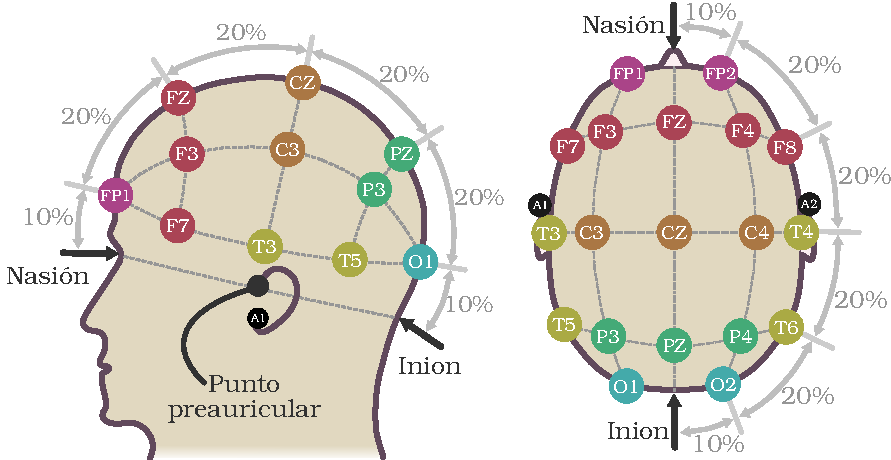
\includegraphics[width=0.9\linewidth]{./img_diagramas/cabeza_proporcionada_color_v2.pdf} 
%\caption{Sistema de referencia 10--20}
\end{figure}
\end{frame}

\begin{frame}\frametitle{Polisomnograma: EOG + EMG}
\begin{figure}
\centering
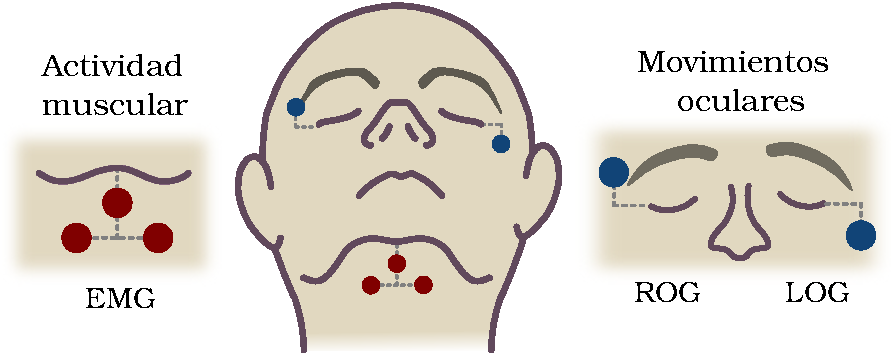
\includegraphics[width=0.9\linewidth]{./img_diagramas/emg_eog_v3.pdf} 
%\caption{Sistema de referencia 10--20}
\end{figure}
\end{frame}

\begin{frame}\frametitle{Registro de PSG}
\begin{figure}
\centering
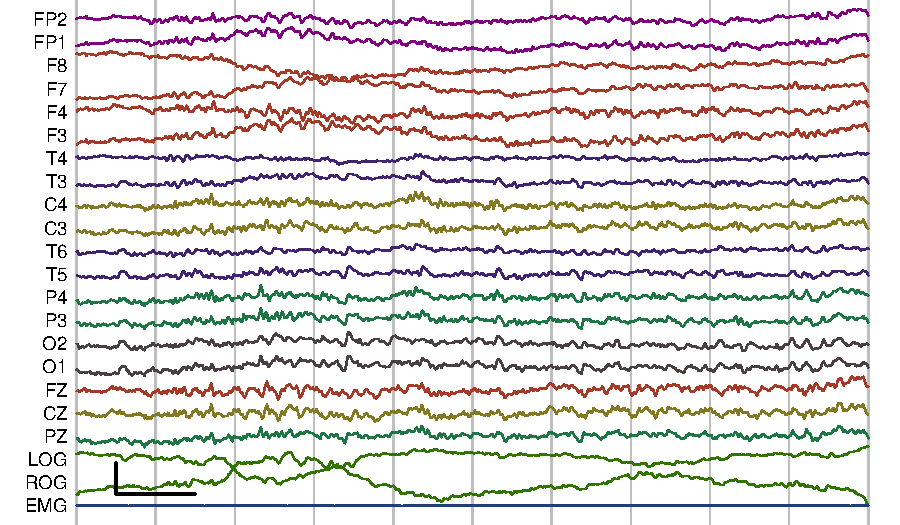
\includegraphics[width=0.9\linewidth]{./img_ejemplos/MJNN_epoca_stam.pdf}
%\caption{PSG: 19 electrodos EEG, 4 electrodos EOG (horizontal y vertical), 2 electrodos EMG en 
%m\'usculos submentonianos}
\end{figure}
\end{frame}

%%%%%%%%%%%%%%%%%%%%%%%%%%%%%%%%%%%%%%%%%%%%%%%%%
%%%%%%%%%%%%%%%%%%%%%%%%%%%%%%%%%%%%%%%%%%%%%%%%%

\begin{frame}\frametitle{Registro de PSG}
\begin{table}
\centering
\bordes{1.1}
\begin{tiny}
\begin{tabular}{llcllcllr}
\toprule
    \phantom{.}&
    &\multirow{2}{*}{\bordes{1}\begin{tabular}{l}Frecuencia de\\ muestreo [Hz]\end{tabular}}
    \bordes{1.2}
    & \multicolumn{2}{c}{Total} & \phantom{l}   & \multicolumn{3}{c}{MOR*}\\
    \cmidrule{4-5}  \cmidrule{7-9}
    &&          &Puntos  &  Tiempo   &&Puntos  &  Tiempo   &  \% \\
\midrule
\multicolumn{6}{l}{\textbf{Grupo CTL}}\\
&VCR &200       &\ppu 5166000 & \ppu  7:10:30 &&\ppu 438000 &   0:36:30 & 8.48 \\
&MJH &512       &    15851520 & \ppu  8:36:00 &&    1950720 &   1:03:30 &12.31 \\
&JAE &512       &    13931520 & \ppu  7:33:30 &&    2626560 &   1:25:30 &18.85 \\
&GHA &200       &\ppu 6558000 & \ppu  9:06:30 &&\ppu 330000 &   0:27:30 & 5.03 \\
&MFGR&200       &\ppu 4932000 & \ppu  6:51:00 &&\ppu 570000 &   0:47:30 &11.56 \\

\rowcolor{gris}
&\multicolumn{1}{c}{$\widehat{\mu}$}  
              & &        & \ppu 7:51:30   &&        &   0:52:06 &11.25 \\
\rowcolor{gris}
&\multicolumn{1}{c}{$\widehat{\sigma}$} 
              & &        & \ppu 0:57:36   &&        &   0:23:00 & 5.13 \\
\midrule

\multicolumn{6}{l}{\textbf{Grupo PDC}}\\
&CLO &512       &    14499840 & \ppu  7:52:00 &&    2027520 &   1:06:00 &13.98 \\
&RLO &512       &    12994560 & \ppu  7:03:00 &&    1520640 &   0:49:30 &11.70 \\
&RRU &200       &\ppu 2484000 & \ppu  3:27:00 &&\ppu 228000 &   0:19:00 & 9.18 \\
&JGZ &512       &    18539520 &      10:03:30 &&\ppu 506880 &   0:16:30 & 2.73 \\
%\rowcolor{gris}
%&\multicolumn{1}{c}{$\widehat{\mu}$}  
%              & &        & \ppu 7:06:23   &&        &   0:37:45 &9.4 \\
%\rowcolor{gris}
%&\multicolumn{1}{c}{$\widehat{\sigma}$} 
%              & &        & \ppu 2:44:55   &&        &   0:24:05 &4.9 \\
&AEFP &512       &    14699520 &       7:58:30 &&\ppu 629760 &   0:20:30 & 4.28 \\

\rowcolor{gris}
&\multicolumn{1}{c}{$\widehat{\mu}$}  
              & &        & \ppu 7:16:48   &&        &   0:34:18 &8.38 \\
\rowcolor{gris}
&\multicolumn{1}{c}{$\widehat{\sigma}$} 
              & &        & \ppu 2:24:43   &&        &   0:22:14 &4.79 \\
\bottomrule
\end{tabular}
\end{tiny}
\end{table}
\end{frame}

\begin{frame}\frametitle{Análisis de estacionariedad}
\begin{itemize}
\item Cada \'epoca fue clasificada \textbf{estacionaria en el sentido de PSR} 
no se rechaza la hip\'otesis de 
estacionariedad ($\alpha < 0.05$)

\item Debido a la variabilidad entre sujetos, se consider\'o la proporci\'on de \'epocas 
estacionarias
% en cada 
%etapa
%\begin{equation*}
%\text{\% \'epocas PE} = \frac{\text{\# \'epocas PE en MOR}}{\text{\# \'epocas en MOR}}
%\end{equation*}

\item El énfasis de las comparaciones es entre MOR y NMOR

%\item Las proporciones se compararon:
%\begin{itemize}
%\item MOR vs NMOR (individual y grupal)
%\item Grupo Control vs Grupo PDC (en cada etapa de sue\~no)
%\end{itemize}
\end{itemize}
\end{frame}

%%%%%%%%%%%%%%%%%%%%%%%%%%%%%%%%%%%%%%%%%%%%%%%%%%%%%%%%%%%%%%%%%%%%%%%%%%%%%%%%%%%%%%%%%%%%%%%%%%%
%%%%%%%%%%%%%%%%%%%%%%%%%%%%%%%%%%%%%%%%%%%%%%%%%%%%%%%%%%%%%%%%%%%%%%%%%%%%%%%%%%%%%%%%%%%%%%%%%%%

\subsection{Patrones visuales}

\begin{frame}\frametitle{Patrones visuales}
\begin{figure}
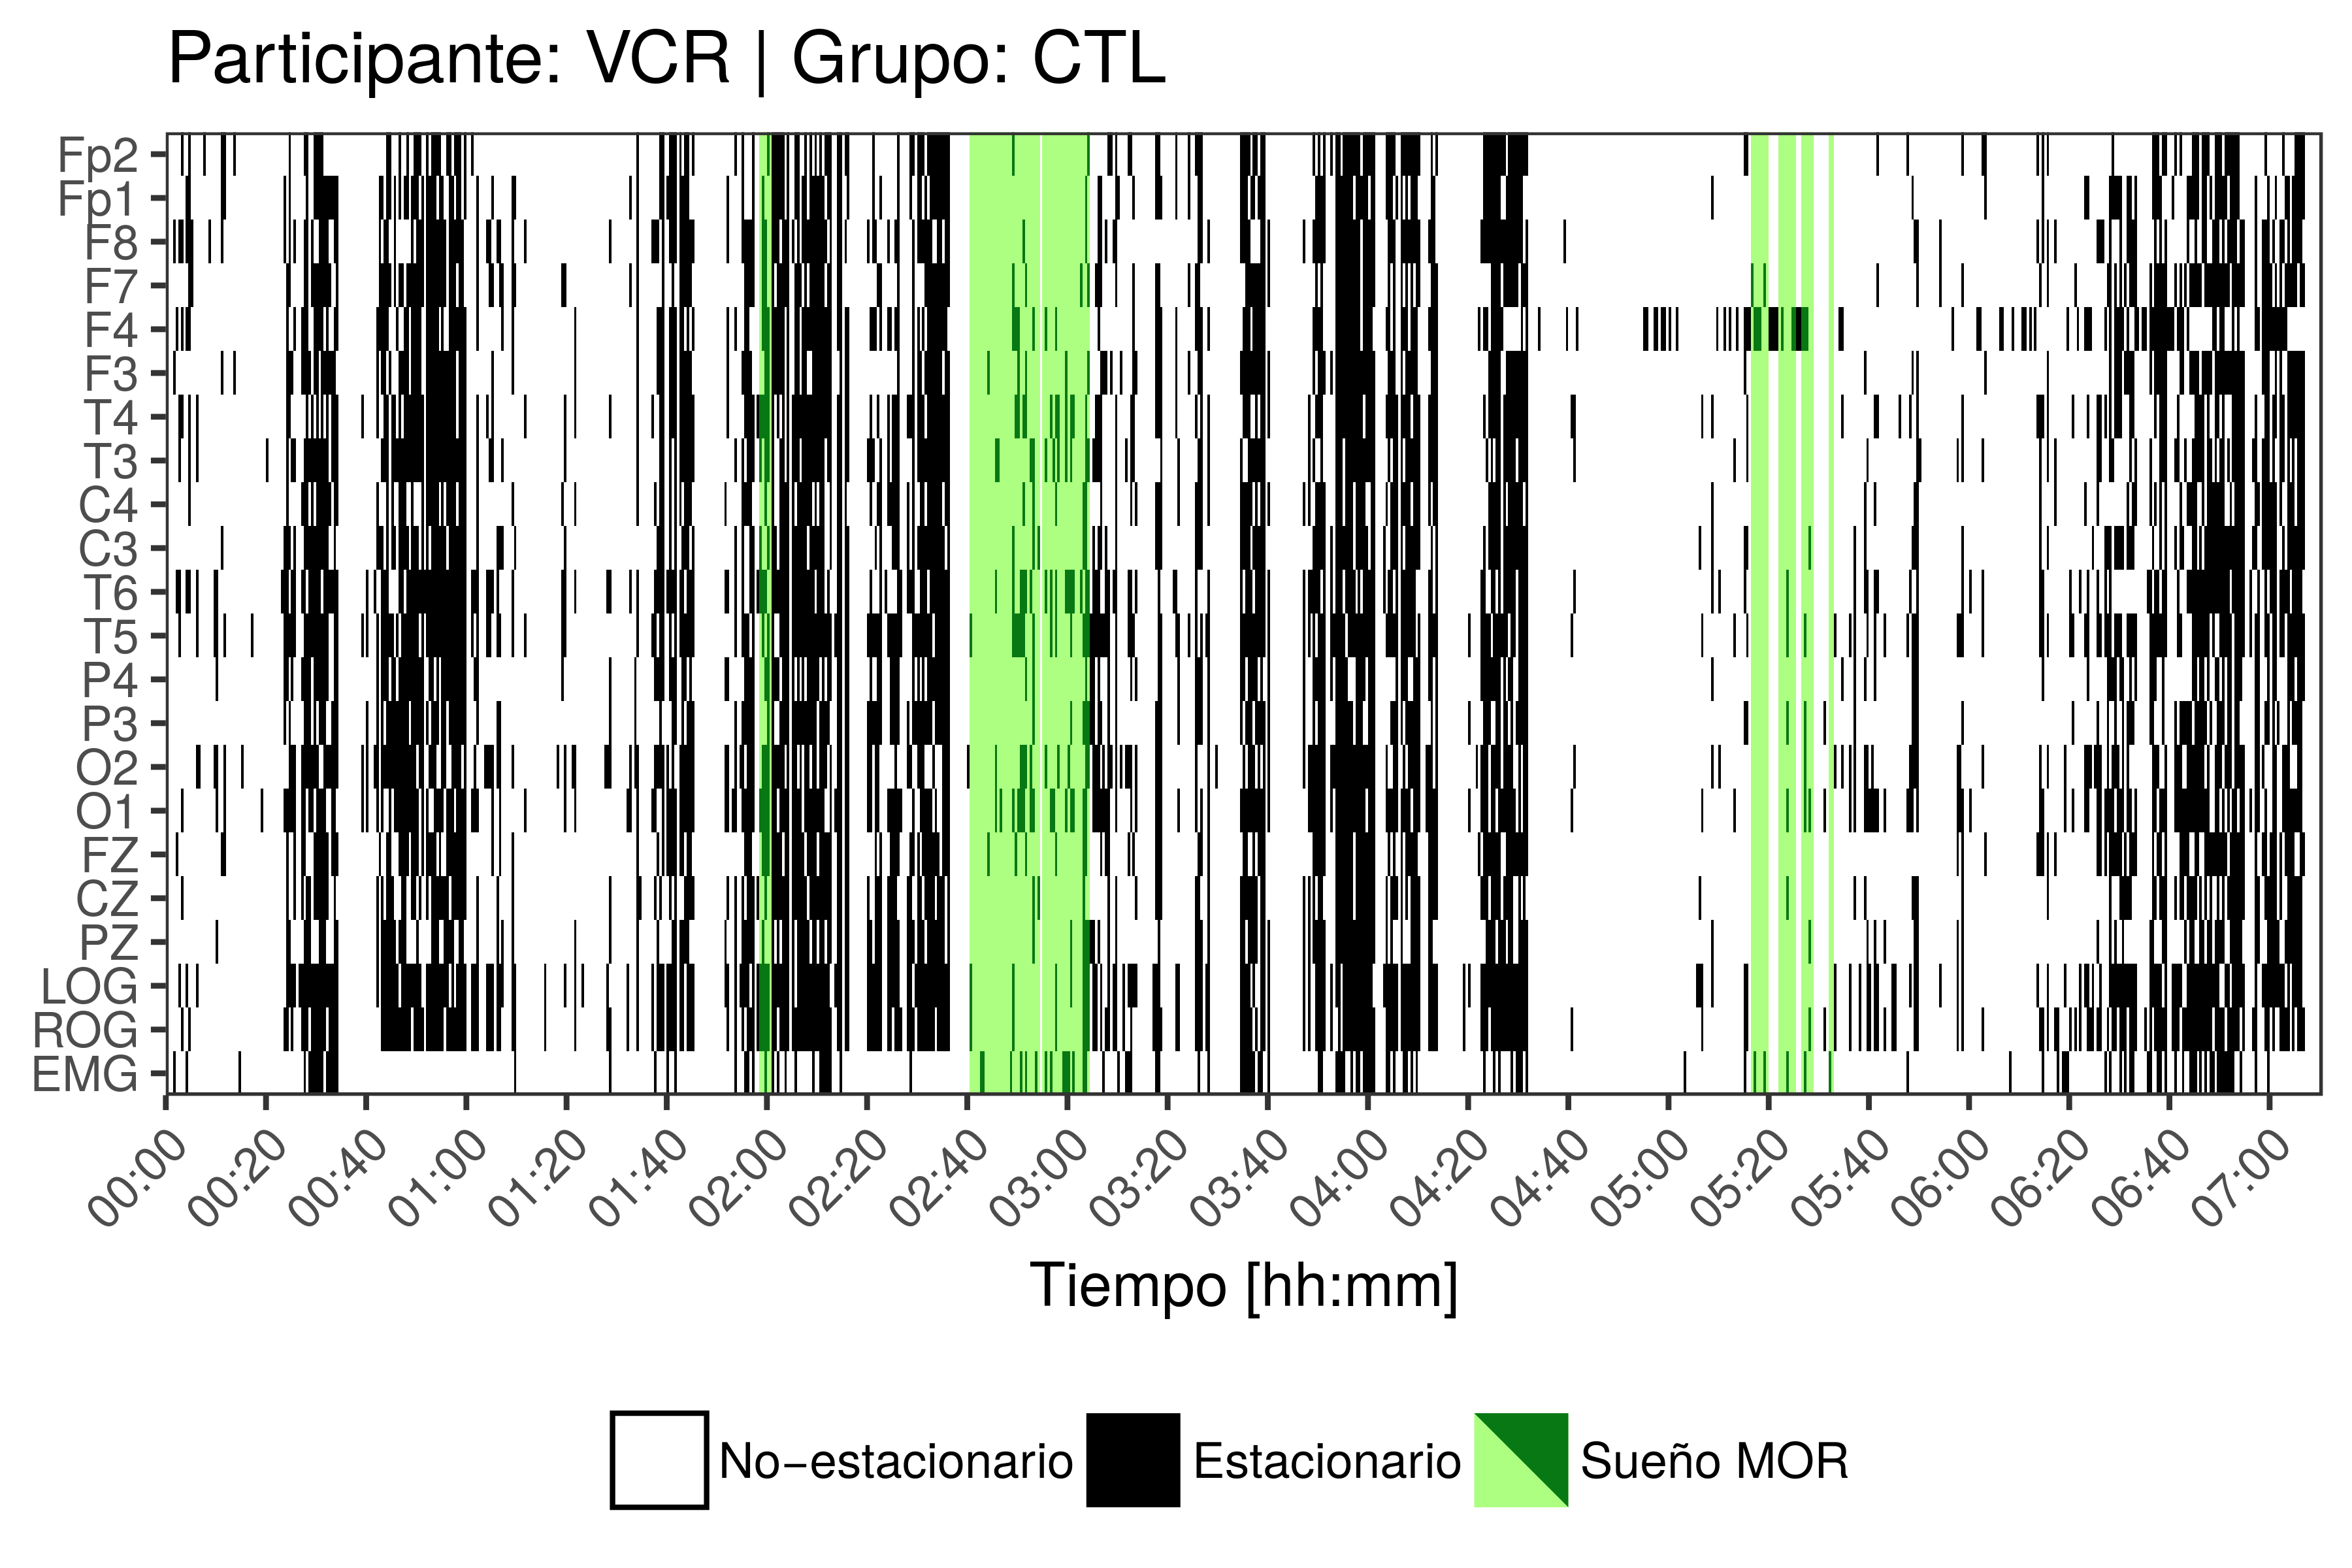
\includegraphics[width=0.95\textwidth]
{./img_art_dfa/zoom_noVCR_v2.png}
%\caption{Disposici\'on gr\'afica para los resultados de la prueba PSR. En verde el sue\~no MOR.}
\end{figure}
\end{frame}

\begin{frame}\frametitle{Patrones visuales}
\begin{figure}
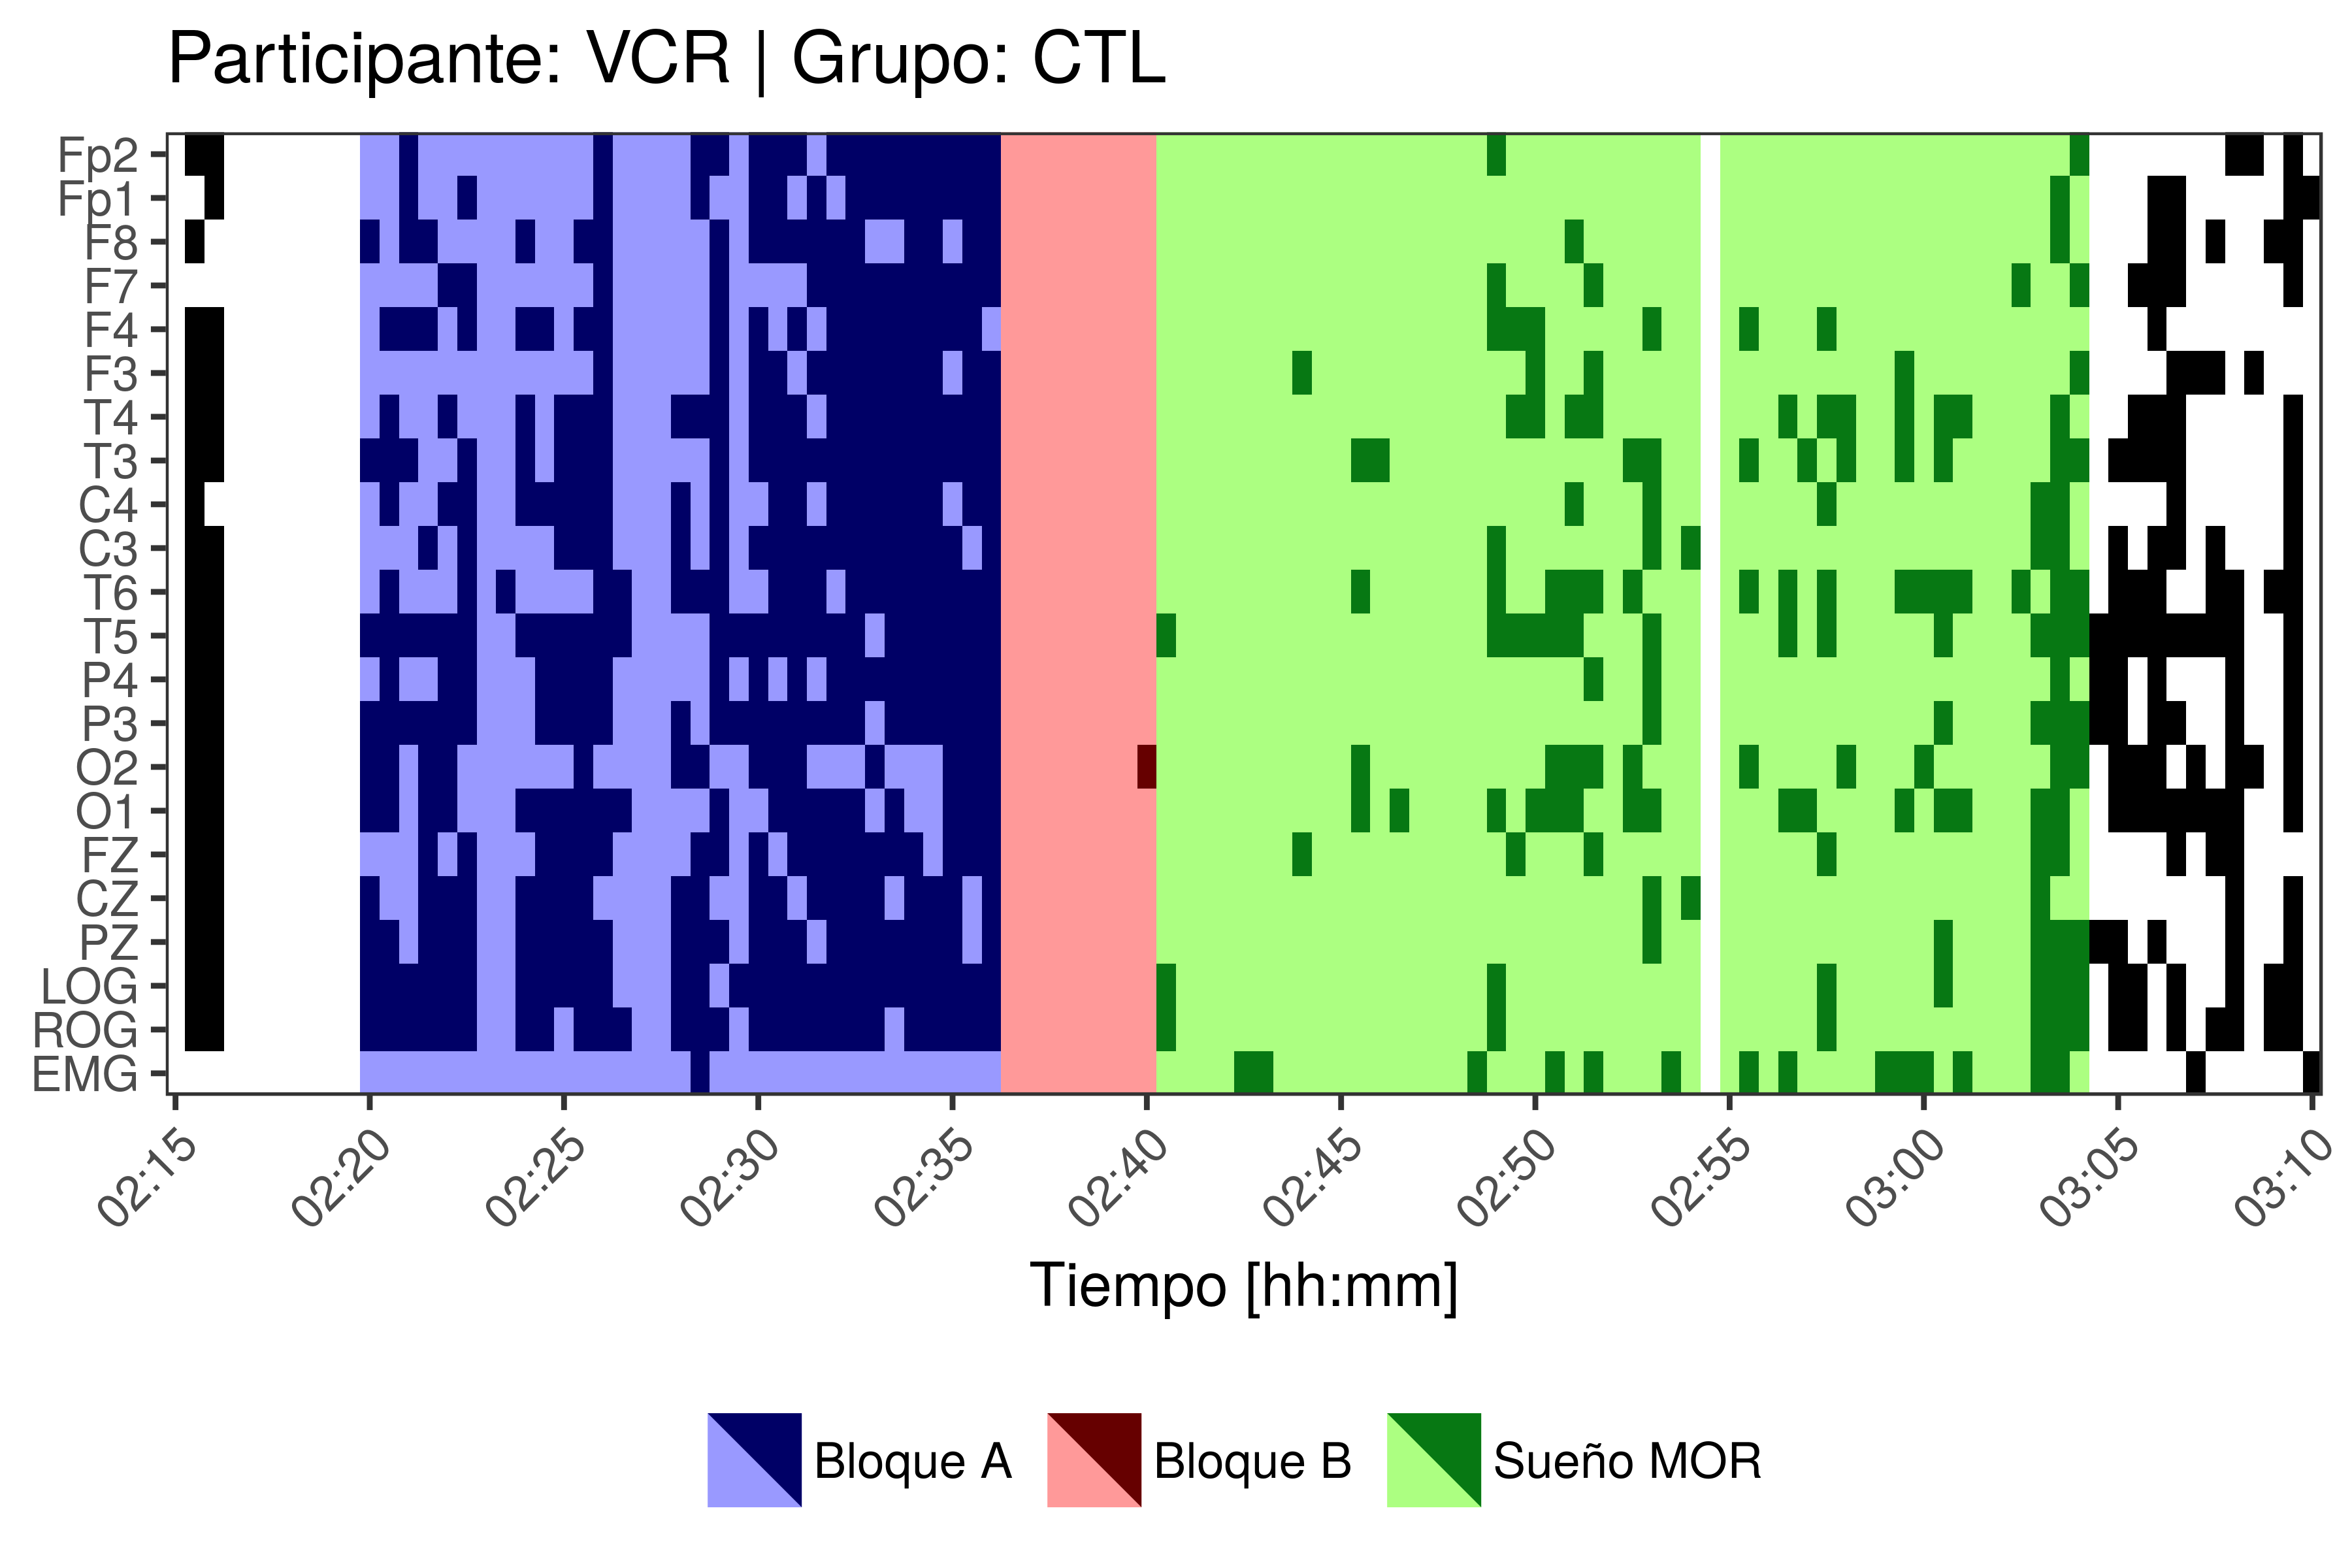
\includegraphics[width=0.95\textwidth]
{./img_art_dfa/zoom_siVCR_v2.png}
%\caption{Disposici\'on gr\'afica para los resultados de la prueba PSR. En verde el sue\~no MOR.}
\end{figure}
\end{frame}

\begin{frame}\frametitle{Diferentes tamaños de ventana}
\begin{figure}
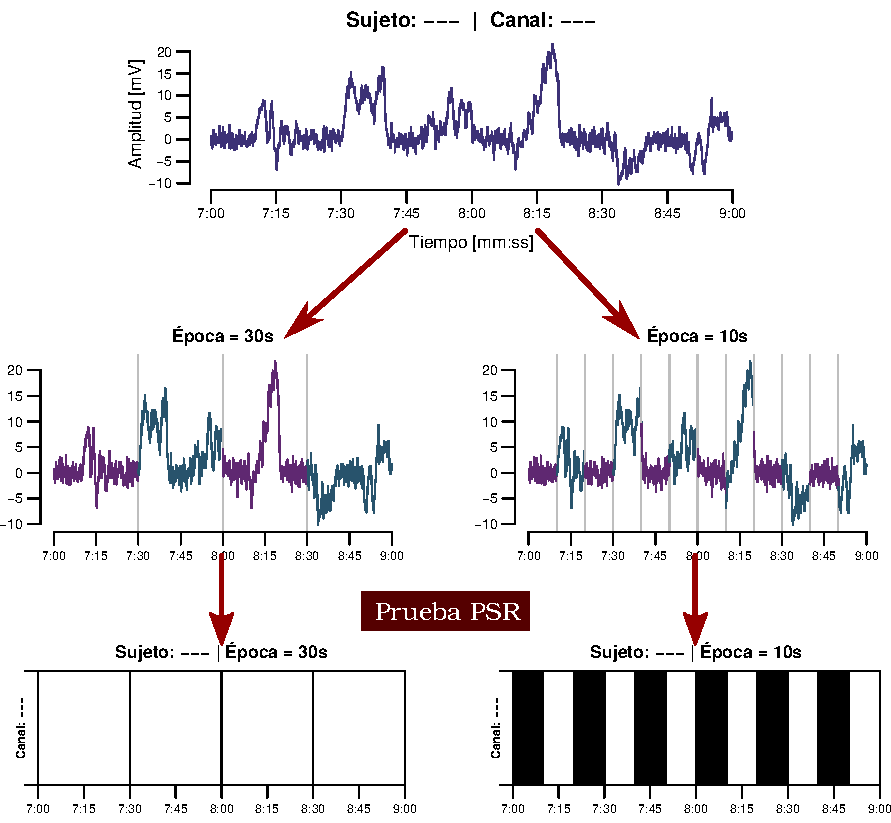
\includegraphics[width=0.95\textwidth]
{./img_diagramas/epocas_diferentes_v2.pdf}
%\caption{Disposici\'on gr\'afica para los resultados de la prueba PSR. En verde el sue\~no MOR.}
\end{figure}
\end{frame}

%\section{Resultados}

%%%%%%%%%%%%%%%%%%%%%%%%%%%%%%%%%%%%%%%%%%%%%%%%%%%%%%%%%%%%%%%%%%%%%%%%%%%%%%%%%%%%%%%%%%%%%%%%%%%

%\subsection{Resultados principales}

%%%%%%%%%%%%%%%%%%%%%%%%%%%%%%%%%%%%%%%%%%%%%%%%%
%%%%%%%%%%%%%%%%%%%%%%%%%%%%%%%%%%%%%%%%%%%%%%%%%

\begin{frame}\frametitle{MOR vs NMOR, individual}
\begin{figure}
\centering
\begin{tabular}{ccccc}
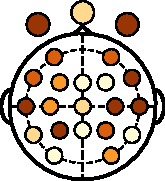
\includegraphics[width=0.15\textwidth]{./img_art_dfa/cabeza_new_VCR_30.pdf} &
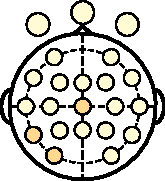
\includegraphics[width=0.15\textwidth]{./img_art_dfa/cabeza_new_MJH_30.pdf} &
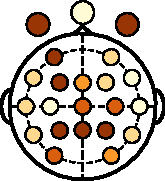
\includegraphics[width=0.15\textwidth]{./img_art_dfa/cabeza_new_JAE_30.pdf} &
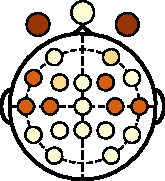
\includegraphics[width=0.15\textwidth]{./img_art_dfa/cabeza_new_GHA_30.pdf} &
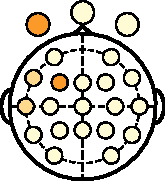
\includegraphics[width=0.15\textwidth]{./img_art_dfa/cabeza_new_MFGR_30.pdf} \\
VCR & MJH & JAE & GHA & MFGR \\
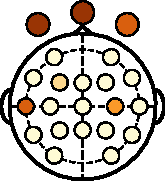
\includegraphics[width=0.15\textwidth]{./img_art_dfa/cabeza_new_CLO_30.pdf} &
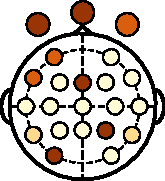
\includegraphics[width=0.15\textwidth]{./img_art_dfa/cabeza_new_RLO_30.pdf} &
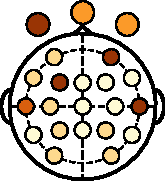
\includegraphics[width=0.15\textwidth]{./img_art_dfa/cabeza_new_RRU_30.pdf} &
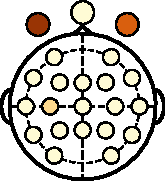
\includegraphics[width=0.15\textwidth]{./img_art_dfa/cabeza_new_JGZ_30.pdf} &
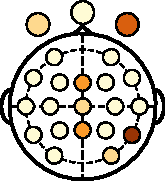
\includegraphics[width=0.15\textwidth]{./img_art_dfa/cabeza_new_AEFP_30.pdf} \\
CLO & RLO & RRU & JGZ & AEFP
\end{tabular}
%\caption{En azul las zonas donde se encontraron diferencias significativas}
\end{figure}
\end{frame}

%%%%%%%%%%%%%%%%%%%%%%%%%%%%%%%%%%%%%%%%%%%%%%%%%
%%%%%%%%%%%%%%%%%%%%%%%%%%%%%%%%%%%%%%%%%%%%%%%%%

\begin{frame}\frametitle{MOR vs NMOR, grupal}
\begin{figure}
\centering
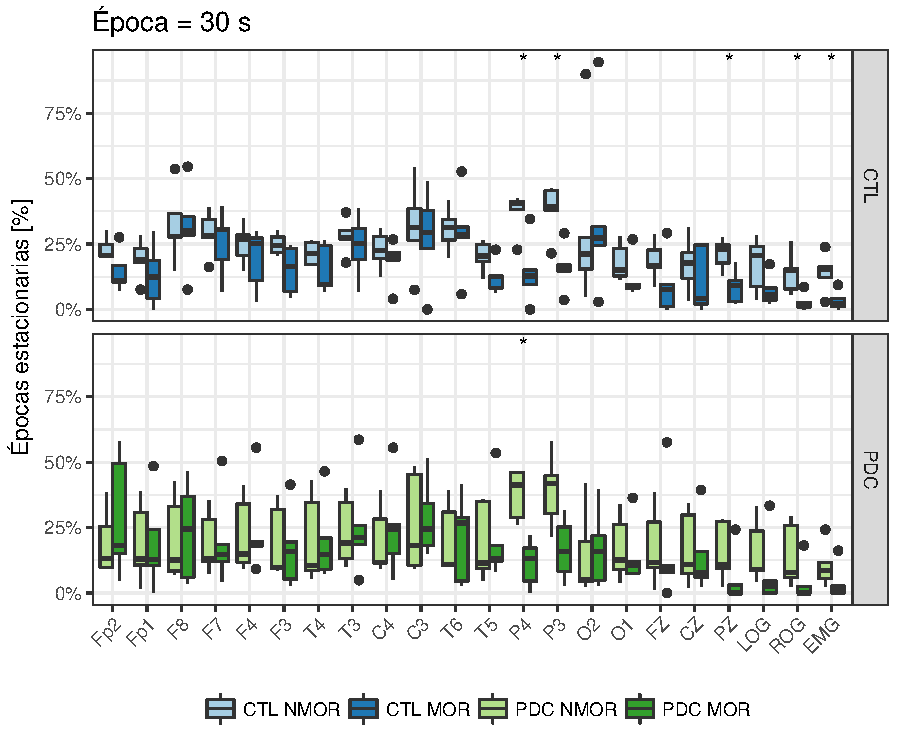
\includegraphics[width=0.8\linewidth]
{./img_art_dfa/Comparacion_gpos_CTL_PDC_v3.pdf} 
%\caption{ Promedio $\pm$ 1 desviaci\'on est\'andar. MOR: verde, NMOR: negro.}
\end{figure}
\end{frame}

\begin{frame}\frametitle{Gpo. Control vs Gpo. PDC}
\begin{figure}
\centering
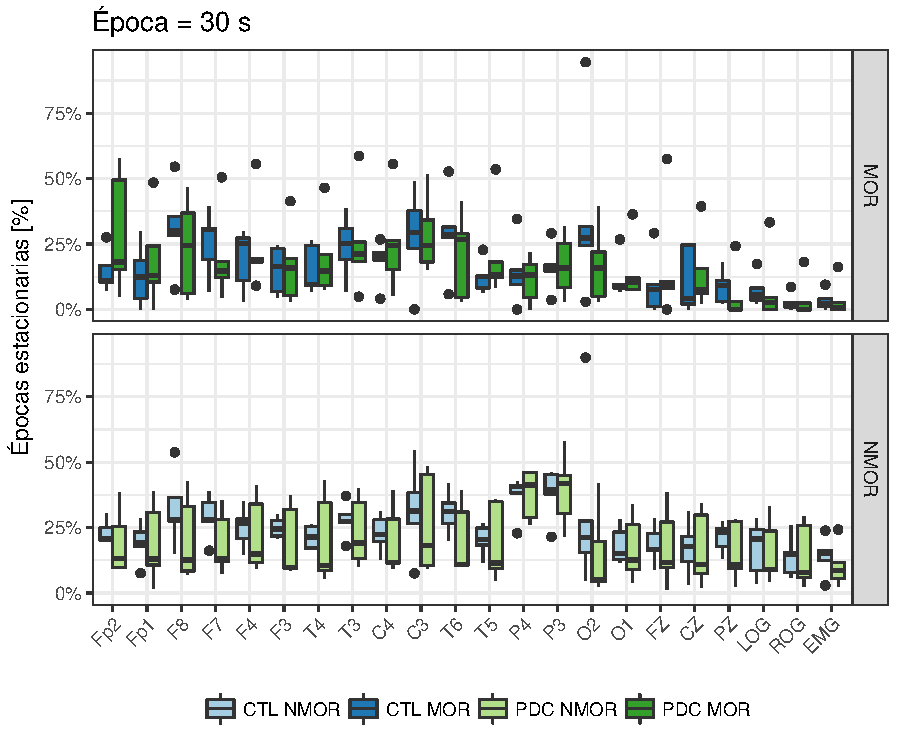
\includegraphics[width=0.8\linewidth]
{./img_art_dfa/Comparacion_gpos_MOR_NMOR_v3.pdf} 
%\caption{ Promedio $\pm$ 1 desviaci\'on est\'andar. Control: azul, PDC: rojo.}
\end{figure}
\end{frame}

%%%%%%%%%%%%%%%%%%%%%%%%%%%%%%%%%%%%%%%%%%%%%%%%%
%%%%%%%%%%%%%%%%%%%%%%%%%%%%%%%%%%%%%%%%%%%%%%%%%

%%%%%%%%%%%%%%%%%%%%%%%%%%%%%%%%%%%%%%%%%%%%%%%%%
%%%%%%%%%%%%%%%%%%%%%%%%%%%%%%%%%%%%%%%%%%%%%%%%%

%\begin{frame}\frametitle{MOR vs NMOR, diferencias significativas}
%\begin{figure}
%\centering
%\includegraphics[width=0.4\linewidth]
%{./img_diagramas/cabecita.pdf} 
%\caption{Sitios con diferencias 
%significativas en la comparaci\'on entre el porcentaje de \'epocas PE durante sue\~no MOR y NMOR, 
%para el grupo Control}
%\end{figure}
%\end{frame}

%%%%%%%%%%%%%%%%%%%%%%%%%%%%%%%%%%%%%%%%%%%%%%%%%
%%%%%%%%%%%%%%%%%%%%%%%%%%%%%%%%%%%%%%%%%%%%%%%%%



%%%%%%%%%%%%%%%%%%%%%%%%%%%%%%%%%%%%%%%%%%%%%%%%%
%%%%%%%%%%%%%%%%%%%%%%%%%%%%%%%%%%%%%%%%%%%%%%%%%

%\begin{frame}%\frametitle{}
%\begin{figure}
%\begin{tabular}{c}
%\includegraphics[width=0.3\textwidth]
%{./img_ejemplos/zoom_VCR.pdf}
%\includegraphics[width=0.3\textwidth]
%{./img_ejemplos/zoom_MJH.pdf}
%\includegraphics[width=0.3\textwidth]
%{./img_ejemplos/zoom_JAE.pdf}
%\\
%\includegraphics[width=0.3\textwidth]
%{./img_ejemplos/zoom_GHA.pdf}
%\includegraphics[width=0.3\textwidth]
%{./img_ejemplos/zoom_MFGR.pdf}
%\end{tabular}
%\caption{Patrones visuales que, se propone, est\'a asociado con la aparici\'on del sue\~no MOR}
%\end{figure}
%\end{frame}

%%%%%%%%%%%%%%%%%%%%%%%%%%%%%%%%%%%%%%%%%%%%%%%%%%%%%%%%%%%%%%%%%%%%%%%%%%%%%%%%%%%%%%%%%%%%%%%%%%%
%%%%%%%%%%%%%%%%%%%%%%%%%%%%%%%%%%%%%%%%%%%%%%%%%%%%%%%%%%%%%%%%%%%%%%%%%%%%%%%%%%%%%%%%%%%%%%%%%%%

\subsection{Discusi\'on}

%\begin{frame}\frametitle{Sobre los sujetos excluidos}
%\begin{figure}
%\centering
%\includegraphics[width=0.95\linewidth]
%{./img_ejemplos/FGHSUE_est.png} 
%\caption{Compilado gr\'afico para el sujeto FGH.}
%\end{figure}
%\end{frame}
%
%%%%%%%%%%%%%%%%%%%%%%%%%%%%%%%%%%%%%%%%%%%%%%%%%%
%%%%%%%%%%%%%%%%%%%%%%%%%%%%%%%%%%%%%%%%%%%%%%%%%%
%
%\begin{frame}\frametitle{Sobre los sujetos excluidos}
%\begin{figure}
%\centering
%\includegraphics[width=0.95\linewidth]
%{./img_ejemplos/FGH_297_PDG_lucirse_PSG.pdf} 
%\caption{Una \'epoca t\'ipica del registro PSG para el sujeto FGH durante sue\~no MOR. }
%\end{figure}
%\end{frame}

%%%%%%%%%%%%%%%%%%%%%%%%%%%%%%%%%%%%%%%%%%%%%%%%%
%%%%%%%%%%%%%%%%%%%%%%%%%%%%%%%%%%%%%%%%%%%%%%%%%

\begin{frame}\frametitle{Sobre el tama\~no de la \'epoca}
\begin{figure}
\centering
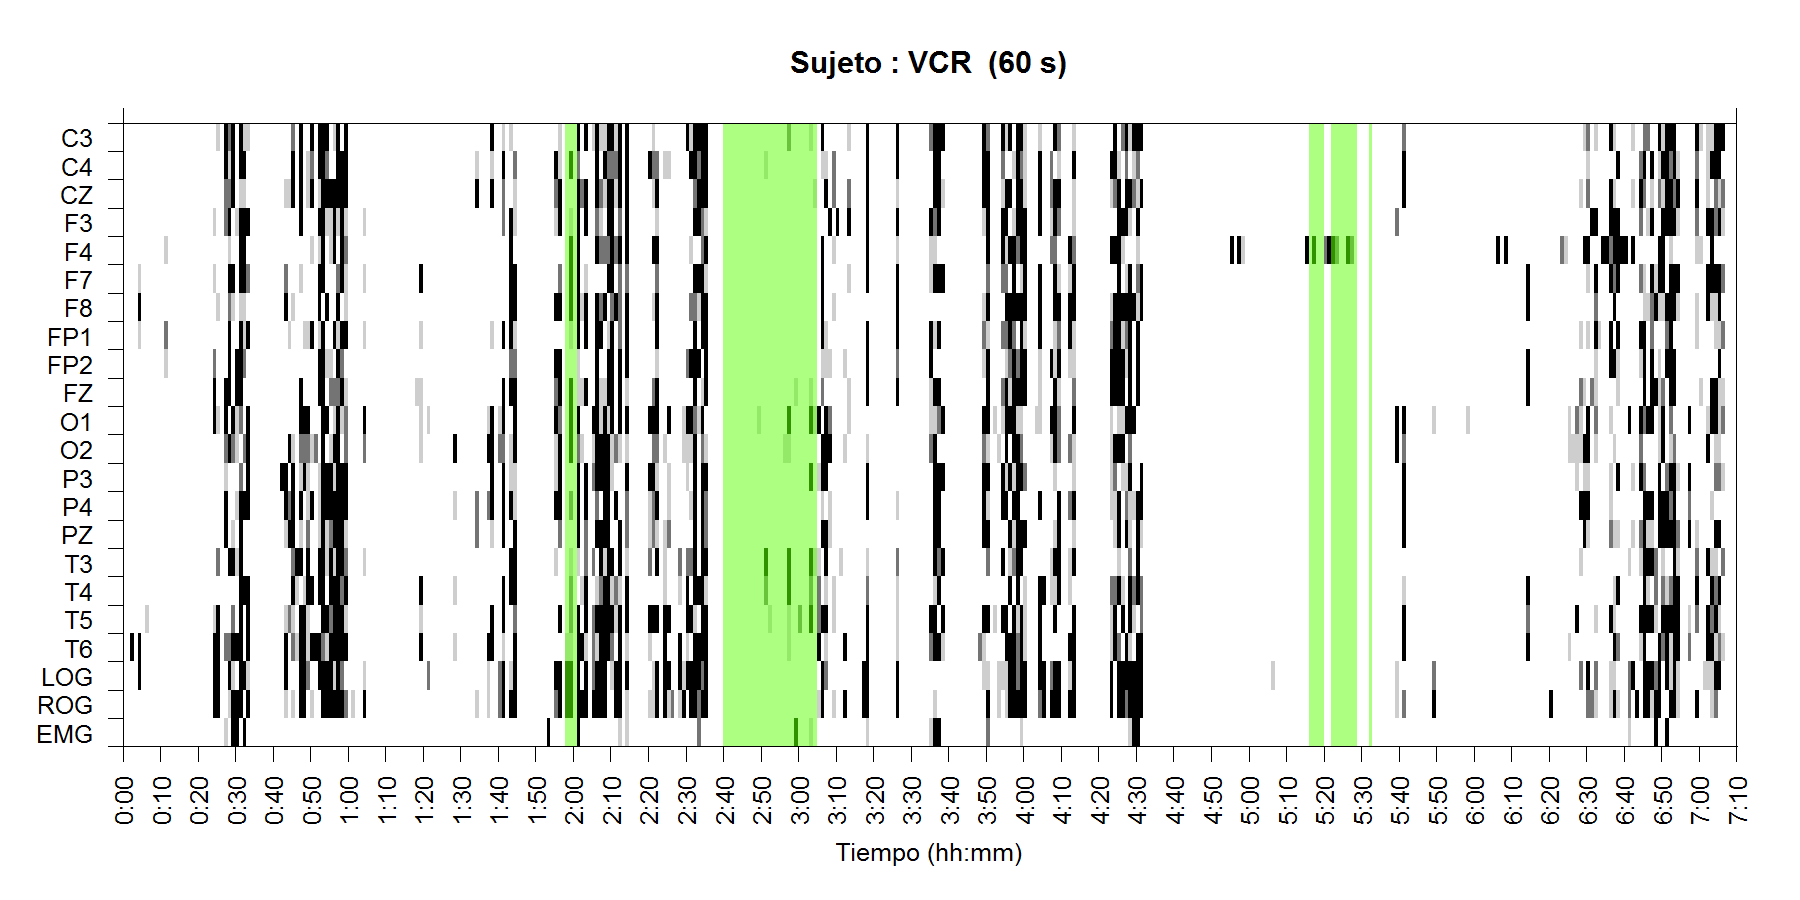
\includegraphics[width=0.9\linewidth]
{./img_ejemplos/VCNNS1_est_60.png} 
\end{figure}
\end{frame}

%%%%%%%%%%%%%%%%%%%%%%%%%%%%%%%%%%%%%%%%%%%%%%%%%
%%%%%%%%%%%%%%%%%%%%%%%%%%%%%%%%%%%%%%%%%%%%%%%%%

\begin{frame}\frametitle{Sobre el tama\~no de la \'epoca}
\begin{figure}
\centering
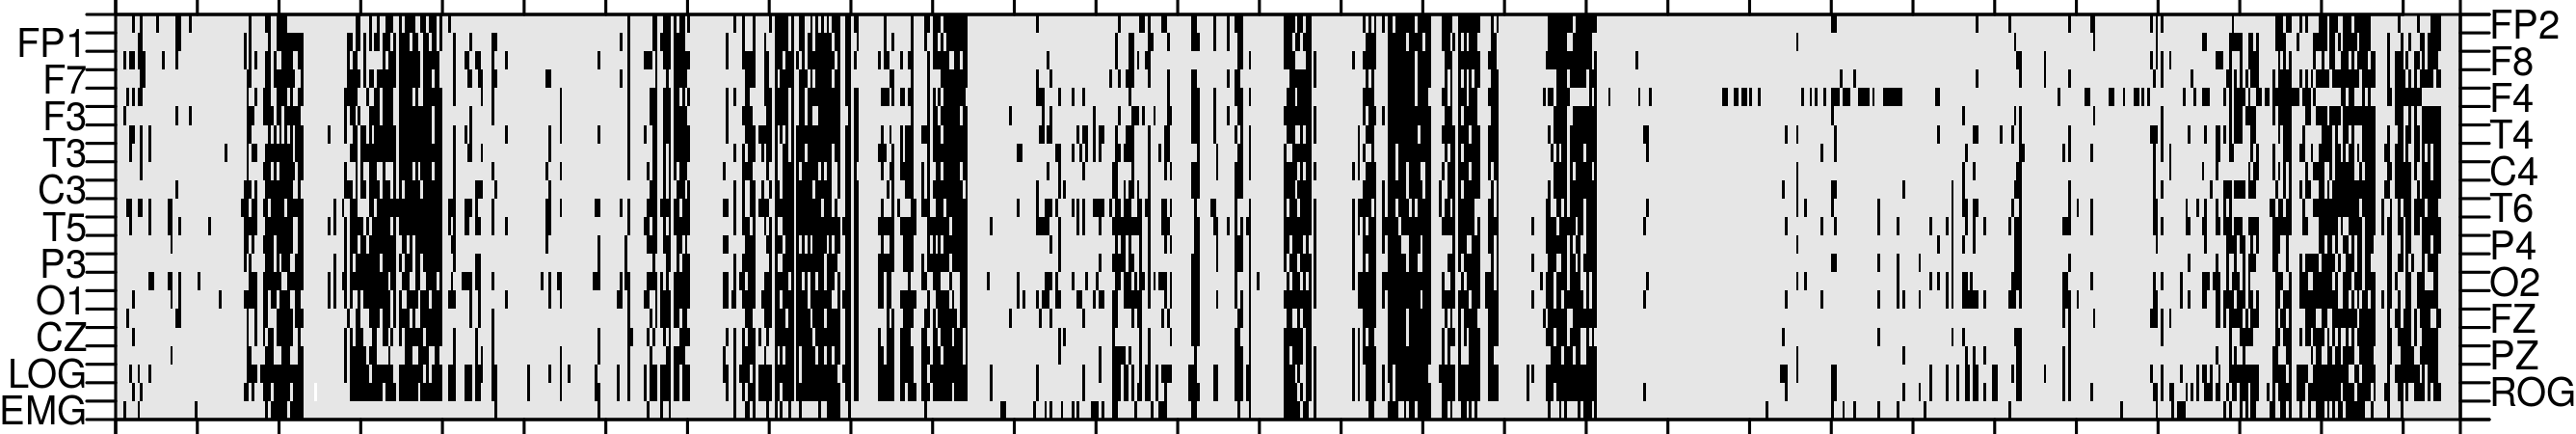
\includegraphics[width=0.9\linewidth]
{./img_ejemplos/VCNNS1_est_30.png} 
\end{figure}
\end{frame}

%%%%%%%%%%%%%%%%%%%%%%%%%%%%%%%%%%%%%%%%%%%%%%%%%
%%%%%%%%%%%%%%%%%%%%%%%%%%%%%%%%%%%%%%%%%%%%%%%%%

\begin{frame}\frametitle{Sobre el tama\~no de la \'epoca}
\begin{figure}
\centering
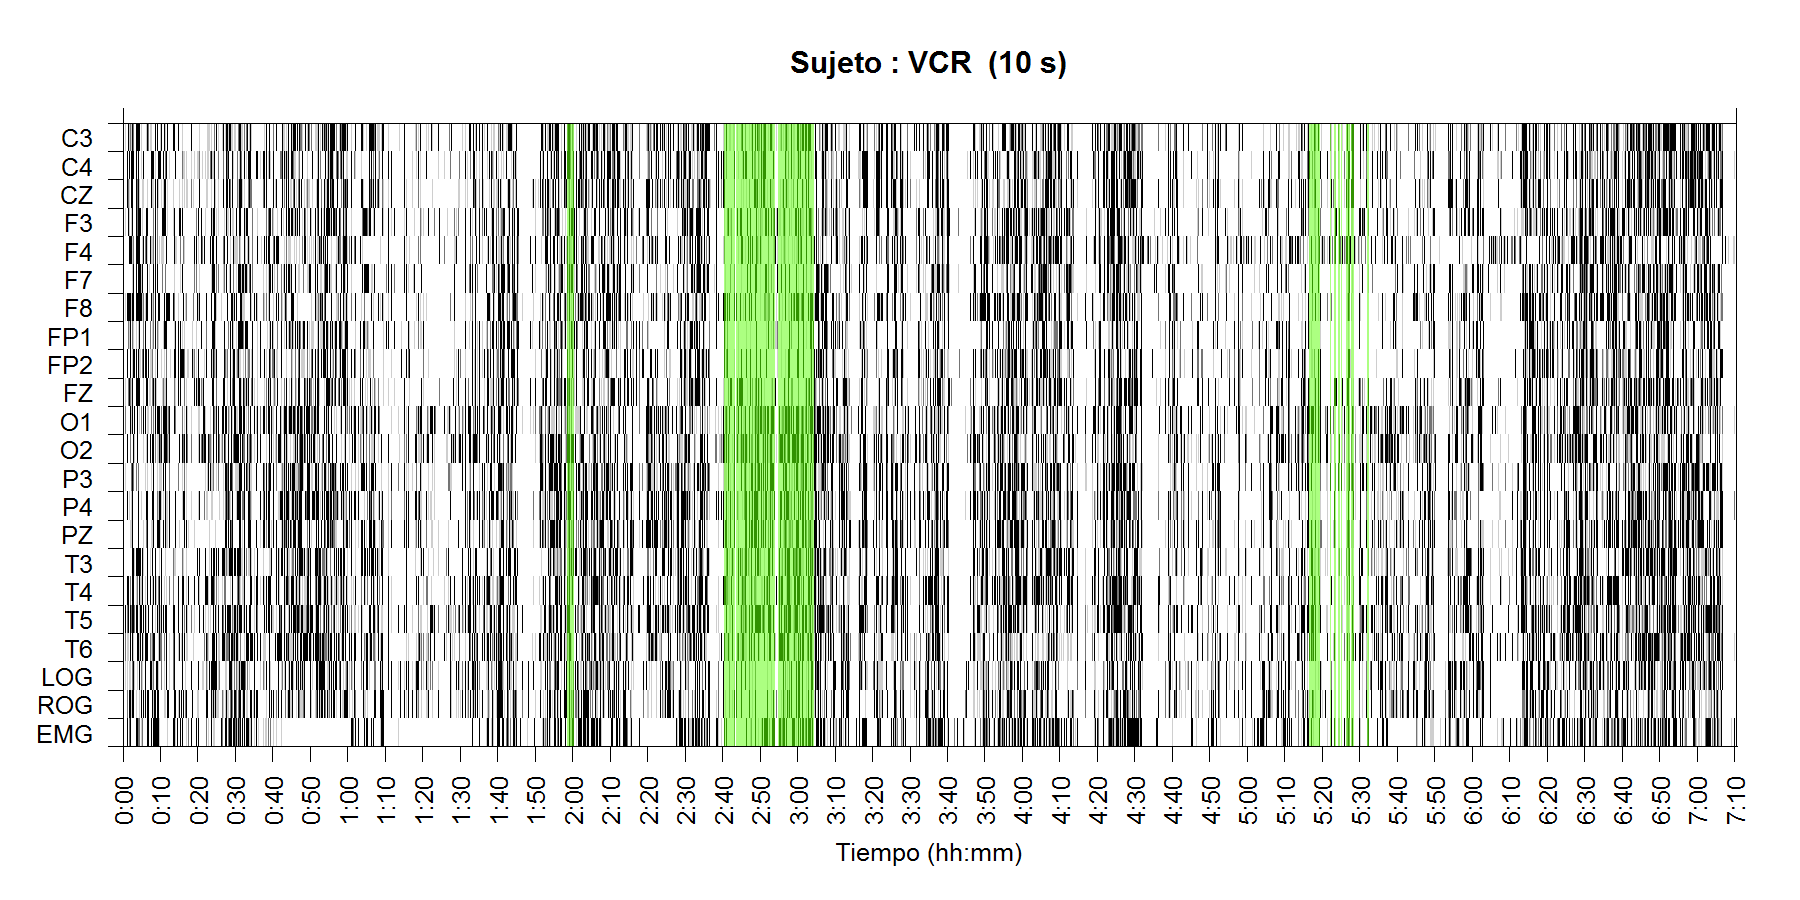
\includegraphics[width=0.9\linewidth]
{./img_ejemplos/VCNNS1_est_10.png} 
\end{figure}
\end{frame}

%%%%%%%%%%%%%%%%%%%%%%%%%%%%%%%%%%%%%%%%%%%%%%%%%
%%%%%%%%%%%%%%%%%%%%%%%%%%%%%%%%%%%%%%%%%%%%%%%%%

\begin{frame}\frametitle{Sobre el tama\~no de la \'epoca}
{\small Estacionariedad local\footcite{Cohen77}}
\begin{figure}
\centering
\begin{tabular}{c}
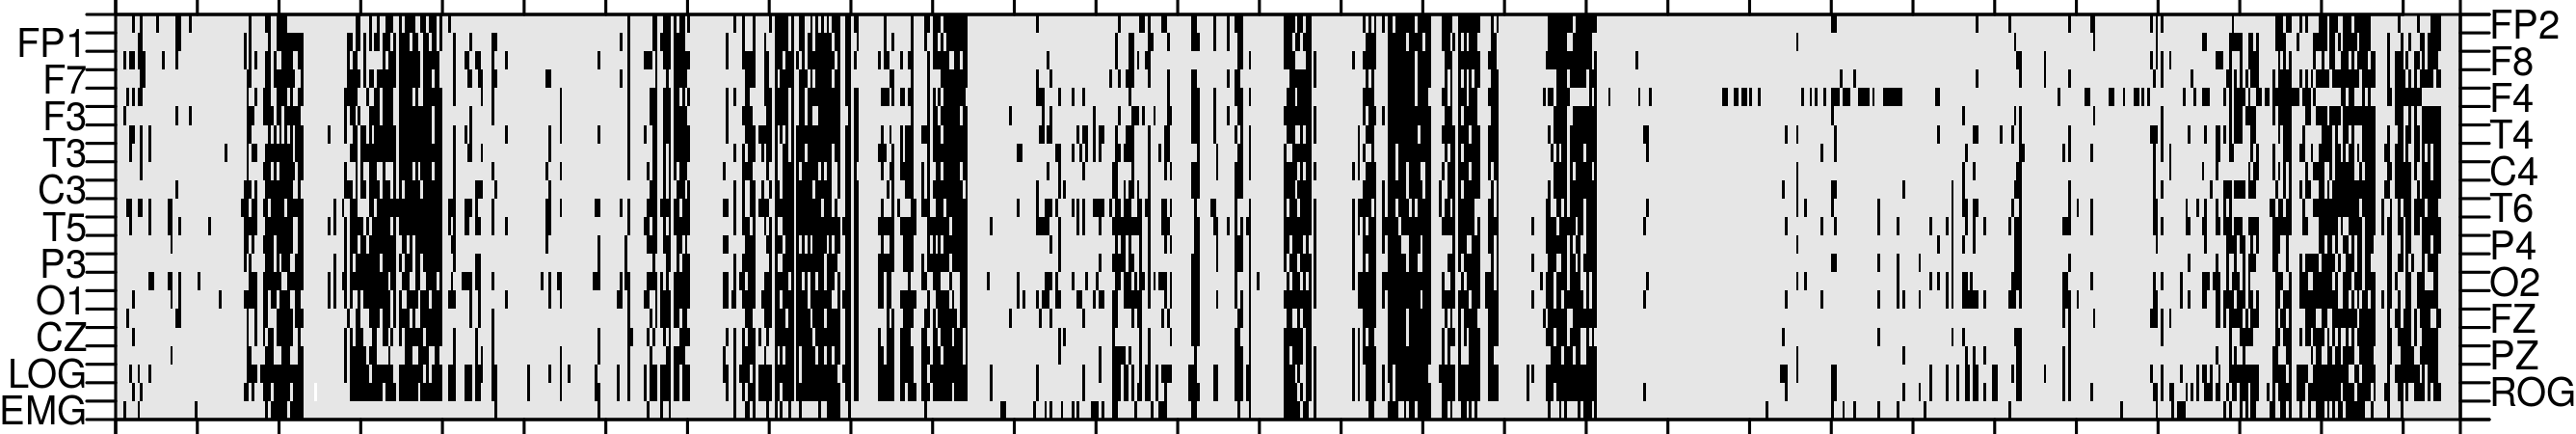
\includegraphics[width=0.4\linewidth]
{./img_ejemplos/VCNNS1_est_30.png} \\
\begin{tabular}{cc}
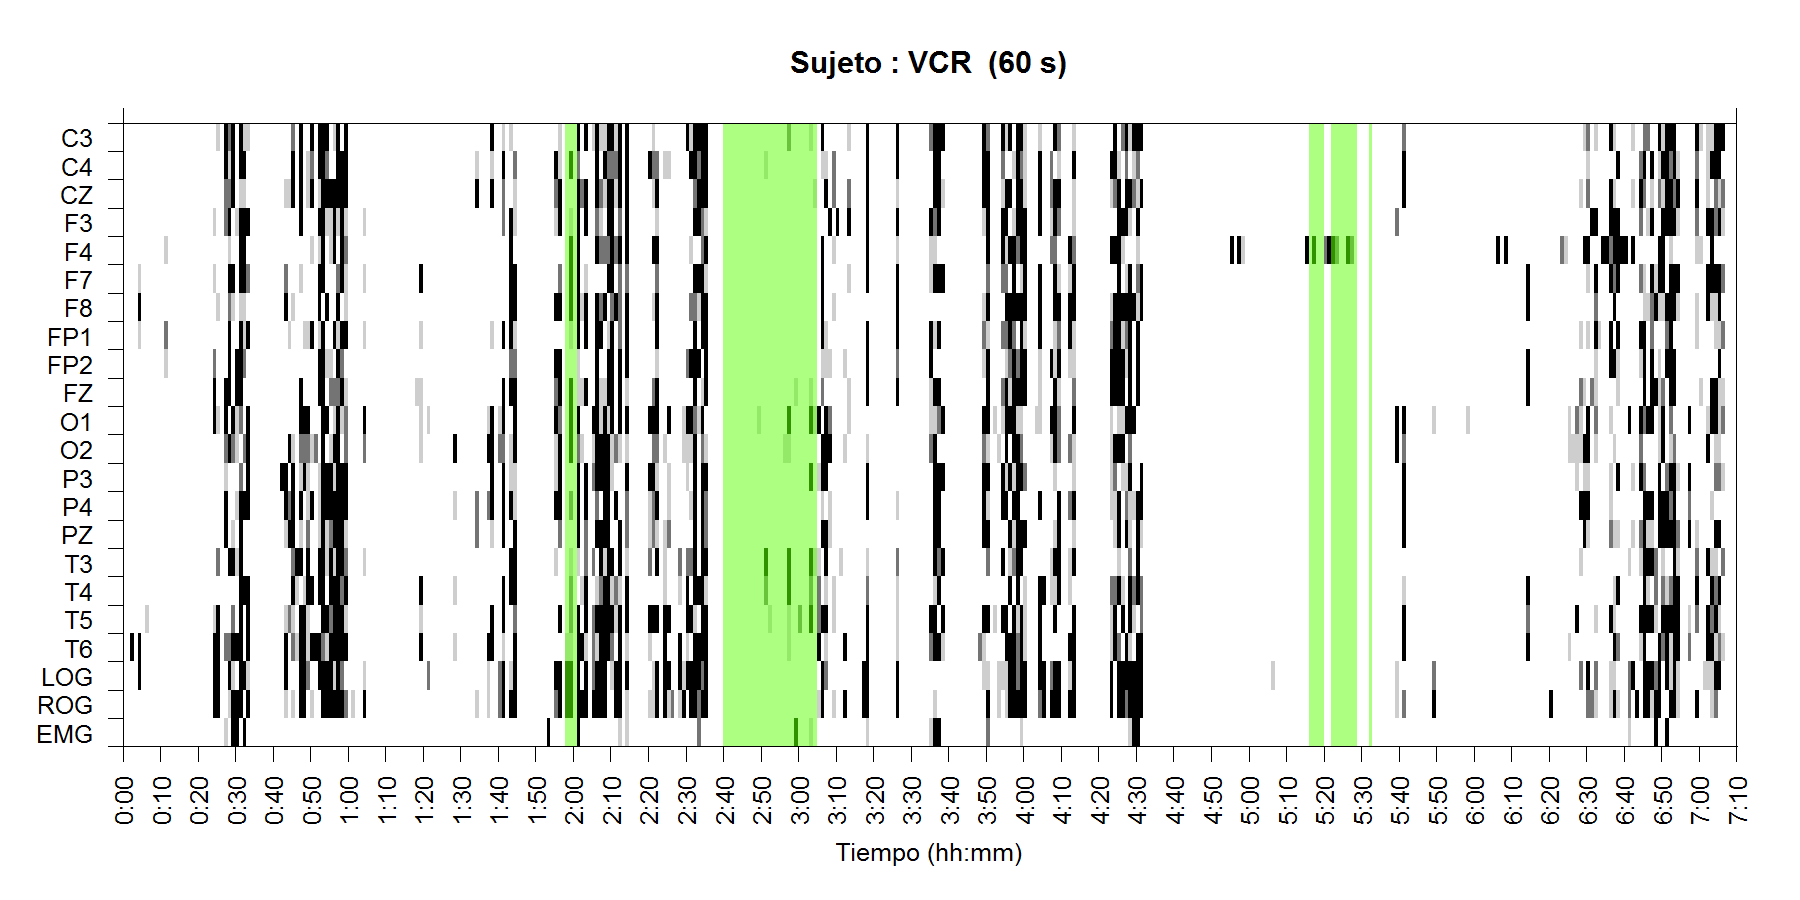
\includegraphics[width=0.4\linewidth]
{./img_ejemplos/VCNNS1_est_60.png} 
&
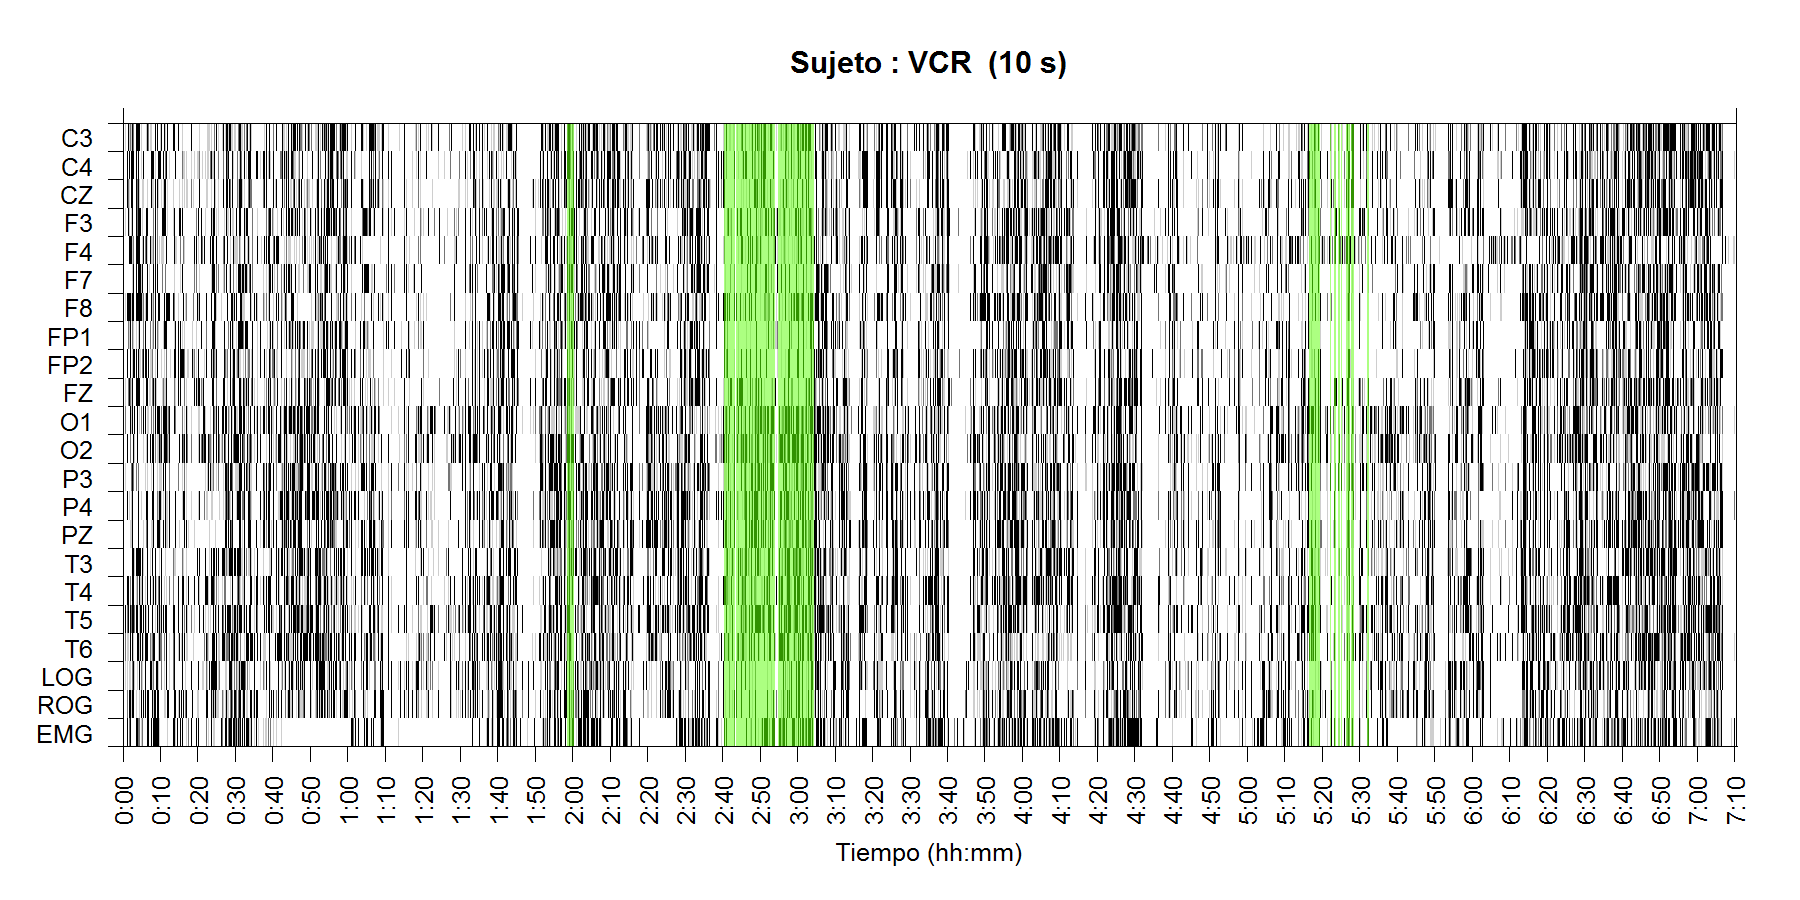
\includegraphics[width=0.4\linewidth]
{./img_ejemplos/VCNNS1_est_10.png} 
\end{tabular}
\end{tabular}
\end{figure}
\end{frame}

%%%%%%%%%%%%%%%%%%%%%%%%%%%%%%%%%%%%%%%%%%%%%%%%%%%%%%%%%%%%%%%%%%%%%%%%%%%%%%%%%%%%%%%%%%%%%%%%%%%
%%%%%%%%%%%%%%%%%%%%%%%%%%%%%%%%%%%%%%%%%%%%%%%%%%%%%%%%%%%%%%%%%%%%%%%%%%%%%%%%%%%%%%%%%%%%%%%%%%%

\subsection{Conclusiones}

\begin{frame}\frametitle{Conclusiones}
\begin{itemize}
\item Presencia proporcional de estacionariedad d\'ebil, significativamente diferente en MOR vs 
NMOR en grupo Control

\item An\'alisis para un AM con par\'alisis facial, detect\'o este padecimiento

\item Consistente con trabajos anteriores %\cite{Valeria}

\item Patrones visuales, predicen parcialmente sue\~no MOR en el grupo Control

\item Registros de PSG en adultos mayores, localmente estacionarias
\end{itemize}
\end{frame}

%%%%%%%%%%%%%%%%%%%%%%%%%%%%%%%%%%%%%%%%%%%%%%%%%%%%%%%%%%%%%%%%%%%%%%%%%%%%%%%%%%%%%%%%%%%%%%%%%%%
%%%%%%%%%%%%%%%%%%%%%%%%%%%%%%%%%%%%%%%%%%%%%%%%%%%%%%%%%%%%%%%%%%%%%%%%%%%%%%%%%%%%%%%%%%%%%%%%%%%

\subsection{Trabajo a futuro}

\begin{frame}\frametitle{Trabajo a futuro}
\begin{itemize}
\item Porcentaje estacionariedad, patrones visuales: marcadores de no-DC

\item Marcador conocido del DC: 'enlentecimiento' de actividad cerebral \footcite{Becerra12} 

\item Prueba de Priestley-Subba Rao: estimadores locales para SDF
\begin{itemize}
\item  Los estimadores usados ¿pueden detectar enlentecimiento?
\end{itemize}

\item Patrones visuales, auxiliares para detecci\'on de MOR en de PSG
\begin{itemize}
\item Identificabilidad de MOR a trav\'es de patrones, ¿marcador cl\'inico?
\end{itemize}
\end{itemize}
\end{frame}


\metroset{background=dark}

\section*{Gracias por su atención}


%%%%%%%%%%%%%%%%%%%%%%%%%%%%%%%%%%%%%%%%%%%%%%%%%

\end{document}

%%%%%%%%%%%%%%%%%%%%%%%%%%%%%%%%%%%%%%%%%%%%%%%%%%%%%%%%%%%%%%%%%%%%%%%%%%%%%%%%%%%%%%%%%%%%%%%%%%%